%\documentclass[12pt]{amsart}
\documentclass[11pt,reqno]{article}
%\usepackage{cases}

%\RequirePackage[numbers]{natbib}
%\RequirePackage[authoryear]{natbib}%% uncomment this for author-year citations
\RequirePackage[colorlinks,citecolor=blue,urlcolor=blue]{hyperref}%% uncomment this for coloring bibliography citations and linked URLs
\RequirePackage{graphicx}%% uncomment this for including figures

\usepackage[
backend=biber,
style=authoryear
]{biblatex}

\addbibresource{references.bib}

\usepackage{setspace}
\usepackage{amsmath}
\usepackage{amssymb}
\usepackage{amscd}
\usepackage{amsthm}
\usepackage{amsfonts}
\usepackage{mathrsfs}
\usepackage{graphicx}
\graphicspath{{figures/}}
\usepackage[perpage,symbol*]{footmisc}
\usepackage{float}
\usepackage{hyperref}
\usepackage{color}  
\usepackage{tikz}
\usepackage{caption}
\usepackage{subcaption}

\usepackage{algorithm2e}

%\usepackage{natbib}
%\bibliographystyle{abbrvnat}
%\setcitestyle{authoryear,open={(},close={)}}
\usepackage{authblk}

\usepackage{csquotes}
\usepackage[english]{babel}

\renewcommand{\baselinestretch}{1.0}
\setlength{\oddsidemargin}{-0.5cm}
\setlength{\evensidemargin}{-0.5cm}
\renewcommand{\topmargin}{-2cm}
\renewcommand{\oddsidemargin}{0mm}
\renewcommand{\evensidemargin}{0mm}
\renewcommand{\textwidth}{180mm}
\renewcommand{\textheight}{240mm}

\DeclareMathOperator*{\argmax}{arg\,max}
\DeclareMathOperator*{\argmin}{arg\,min}
\newcommand{\T}{\intercal}
\newcommand{\commentout}[1]{}

\newcommand{\kmedit}[1]{{\color{purple}  #1}}
\newcommand{\meng}[1]{{\color{purple} \sf $\clubsuit\clubsuit\clubsuit$ Kun Meng: [#1]}}
\newcommand{\Meng}[1]{\margMa{(Kun Meng) #1}}

\newcommand{\zielinski}[1]{{\color{blue} \sf $\spadesuit\spadesuit\spadesuit$ Rob Zielinski: [#1]}}

\theoremstyle{definition}
\newtheorem{definition}{Definition}
\newtheorem{theorem}{Theorem}

\begin{document}

\title{Longitudinal Principal Manifold Estimation}
\author[1]{Robert Zielinski}
\author[2]{Kun Meng}
\author[1]{Ani Eloyan}
\affil[1]{Department of Biostatistics, Brown University}
\affil[2]{Division of Applied Mathematics, Brown University}



\maketitle

\doublespacing

\section*{Abstract}

\section{Introduction}

Neuroimaging plays a critical role in the diagnosis and monitoring of a number of common neurodegenerative conditions, such as Alzheimer's disease (AD) and Parkinson's disease (\cite{knopmanAlzheimerDisease2021}, \cite{poeweParkinsonDisease2017}). Frequently, interest centers around longitudinal changes in one or more neurological substructures. These structural changes can be observed in magnetic resonance imaging (MRI) data (\cite{crainiceanu2016tutorial}). For example, it is common to observe atrophy in the hippocampus, a structure in the temporal lobe of the brain, of those with AD or cognitive impairment related to other causes. Image segmentation allows for the extraction of subcortical structures from MRI images of the brain for further analysis.

Traditionally, manual segmentation of images by a trained radiologist has been considered the most accurate approach for segmentation of regions of interest and is the gold standard. However, this approach is highly time and resource intensive. In studies analyzing a large number of images, this approach may impose prohibitive costs. Additionally, manual segmentation suffers from meaningful inter-rater and intra-rater variability (\cite{boccardiSurveyProtocolsManual2011}). Automated segmentation approaches, such as FSL-FIRST and FreeSurfer, have been introduced to address these concerns (\cite{patenaudeBayesianModelShape2011}, \cite{reuterWithinsubjectTemplateEstimation2012}). While automating the segmentation process drastically reduces costs, it potentially introduces additional inaccuracies.

To anecdotally demonstrate the potential extent of the inaccuracies introduced by segmentation, using FIRST to segment the hippocampus in images of one healthy individual over the course of four years in the Alzheimer's Disease Neuroimaging Initiative (ADNI) dataset, the volume of the left and right hippocampus decreased by 3.6\% and 5.4\%, respectively, but each hippocampus was estimated to have increased in volume between subsequent study visits twice. In a larger comparison of the accuracy of FIRST and FreeSurfer, \cite{mulderHippocampalVolumeChange2014} found that 6.9\% of segmentations by FIRST failed visual inspection for accuracy, as did 7.5\% of segmentations by FreeSurfer. After removing these failed segmentations, FIRST and FreeSurfer produced segmentations with variability similar to and slightly lower than manual segmentation, respectively. If failed segmentations were not removed from analysis, reflecting a more realistic situation when working with a large number of images, variability as measured by the Limits of Agreement were much higher for FIRST and FreeSurfer than for manual segmentation. \cite{mulderHippocampalVolumeChange2014} also found slightly higher rates of segmentation failure among individuals with Alzheimer's disease for both automated segmentation approaches, suggesting that variability increases as images are taken from individuals with greater deviations from the healthy brains on which the segmentation models were trained [See original articles to confirm, see if there are any confirming studies].

Ultimately, high levels of variability are present at the subcortical level, both between study visits for the same individual and between individuals, regardless of the segmentation approach used, and may be particularly influential when using automated segmentation methods. Mitigating the extent of this variability is a priority from a statistical perspective. To this end, in this article, we propose a manifold learning-based method to develop smooth estimates of the surfaces of subcortical structures over time. Manifold learning describes a set of statistical approaches to modeling high-dimensional data that are assumed to lie along a low-dimensional manifold. In medical imaging applications, interacting with a low-dimensional interpretation of a structure may be more intuitive than working with the structure in its original high-dimensional space. For example, \cite{yueParameterizationWhiteMatter2016} seeks to compute a parametric representation of the corpus callosum. To obtain the low-dimensional parameterization of the substructures of interest, the proposed approach extends the principal manifold estimation approach introduced by \cite{mengPrincipalManifoldEstimation2021}.

Previously introduced methods for manifold learning, such as Isomap (\cite{tenenbaumGlobalGeometricFramework2000}), locally linear embedding (\cite{roweisNonlinearDimensionalityReduction2000}), and Laplacian eigenmaps (\cite{belkinLaplacianEigenmapsDimensionality2003a}), are ill-equipped to reach meaningful estimates across multiple time points. This is because these methods consider time as an additional dimension in the data, meaning they include time in the dimension reduction process. This treatment of the time dimension causes it to be incorporated into the low-dimensional parameterization, preventing meaningful interpretation of this dimension. Here, we propose an alternative approach to estimating manifolds over time.

Rather than include time as another dimension in a manifold learning method, we use a process that maintains the interpretability of the time dimension. Specifically, we use the method proposed in \cite{mengPrincipalManifoldEstimation2021} to estimate the appropriate principal manifold at each given time point. We then smooth over these approximated manifolds in the time dimension, yielding an estimate showing longitudinal changes in the underlying manifold. The regularization involved in this process mitigates the effects of variability between study visits.

Some previous work has been conducted on longitudinal dimension reduction methods, but this research has primarily focused on linear methods, such as the longitudinal principal component analysis approach proposed by \cite{kinsonLongitudinalPrincipalComponent2020}. To our knowledge, the approach to longitudinal smoothing in the manifold learning setting taken in this article is novel.

The remainder of this article is laid out as follows: In Section 2, we review the principal manifold framework proposed in \cite{mengPrincipalManifoldEstimation2021}. Section 3 discusses how this approach can be adapted for longitudinal settings, and shows the algorithm being used to accomplish this. Section 4 demonstrates the performance of this approach on simulated data. In Section 5, we apply this method to longitudinal data of the hippocampus in individuals with Alzheimer's disease. The article concludes with a discussion of the method's contributions in Section 6.

\section{Principal Manifolds and Estimation Algorithm}

The framework for principal manifolds originated with the concept of principal curves (PS, \cite{hastiePrincipalCurves1989}), which are essentially curves that pass through the middle of the data. However, the PS framework in \cite{hastiePrincipalCurves1989} is flawed by the model complexity selection, which \cite{duchamp1996extremal} pointed out. Motivated by the penalization approaches in \cite{kegl2000learning} and \cite{smolaRegularizedPrincipalManifolds2001}, \cite{mengPrincipalManifoldEstimation2021} proposed the principal manifold estimation (PME) framework and algorithm. Since our LPME is based on the PME, we review the PME in this section for the audience's convenience. The following concepts and notations are necessary for both the PME and our proposed LPME, and they will be used throughout this paper
\begin{itemize}
\item $d$ and $D$ are two positive integers denoting the dimensions of the low-dimensional manifold and high-dimensional space, respectively; 
\item for any positive integer $q$ and point $\xi=(\xi_1,\ldots,\xi_q)\in\mathbb{R}^q$, $\Vert \xi\Vert_{\mathbb{R}^q}=\sqrt{\sum_{l=1}^q \xi_l^2}$;
    \item $\mathcal{C}_{\infty}(\mathbb{R}^{d} \to \mathbb{R}^{D}) = \left\{f \in \mathcal{C}(\mathbb{R}^{d} \to \mathbb{R}^{D}): \lim_{\|r\|_{\mathbb{R}^{d}} \to \infty}\|f(r)\|_{\mathbb{R}^{D}} = \infty\right\}$, where $\mathcal{C}(\mathbb{R}^{d} \to \mathbb{R}^{D})$ denotes the collection of continuous vector-valued functions mapping from $\mathbb{R}^d$ to $\mathbb{R}^D$; 
    \item for every $f\in \mathcal{C}_{\infty}(\mathbb{R}^{d} \to \mathbb{R}^{D})$, the image of $f$ is referred to as the $d$-dimensional manifold $M_f^d$ determined by $f$, i.e., $M_f^d=\{f(r):\,r\in\mathbb{R}^d\}$;
    \item For each $f\in \mathcal{C}_{\infty}(\mathbb{R}^{d} \to \mathbb{R}^{D})$ and each point $x\in\mathbb{R}^D$, $\pi_f(x)$ is a point in $\mathbb{R}^d$ and denotes the ``projection index" of $x$; roughly, $\pi_f(x)$ is a point in $d$-dimensional space such that $f(\pi_f(x))$ is the projection of $x$ on the manifold $M_f^d$; $\pi_f(x)$ is a generalization of the counterpart in \cite{hastiePrincipalCurves1989}, and its details can be found in Section 2 of \cite{mengPrincipalManifoldEstimation2021};
    \item suppose $u(r_1,\ldots,r_d)$ is a scalar-valued function defined on $\mathbb{R}^d$; $\nabla^{\otimes 2}u=\left(\frac{\partial^2 u}{\partial r_i \partial r_j}\right)_{1\le i,j\le d}$ denotes the Hessian matrix of $u$, and $\|\nabla^{\otimes 2}u\|_{\mathbb{R}^{d \times d}}$ is the function $r \to \|\nabla^{\otimes 2} u(r)\|_{\mathbb{R}^{d \times d}} = \left(\sum_{i, j = 1}^{d}\left|\frac{\partial^2 u}{\partial r_i \partial r_j}(r)\right|^2\right)^{\frac{1}{2}}$; in addition, $\|\nabla^{\otimes 2} u\|_{L^2(\mathbb{R}^{d})}^2 = \int_{\mathbb{R}^{d}}\sum_{i, j = 1}^{d}\left|\frac{\partial^2 u}{\partial r_i \partial r_j}(r)\right|^2dr $, and 
    \begin{align*}
        \nabla^{-\otimes 2}L^2(\mathbb{R}^{d}) = \left\{u \in \mathcal{D}'(\mathbb{R}^{d}): \|\nabla^{\otimes 2} u\|_{\mathbb{R}^{d \times d}} \in L^2(\mathbb{R}^{d})\right\},
    \end{align*}
    where $\mathcal{D}'$ denotes the collection of distributions (also known as generalized functions, see \cite{duchon1977splines} and Chapter 6 of \cite{rudin1991functional});
    \item $\nabla^{-\otimes 2}L^2(\mathbb{R}^{d}\rightarrow\mathbb{R}^D)$ denotes the collection of vector-valued functions $f(r)=\left(f_1(r),\ldots,f_D(r)\right)^\T$ whose components are in $\nabla^{-\otimes 2}L^2(\mathbb{R}^{d})$; besides, $\mathcal{C}_\infty\bigcap\nabla^{-\otimes 2}L^2(\mathbb{R}^{d}\rightarrow\mathbb{R}^D)=\mathcal{C}_\infty(\mathbb{R}^{d}\rightarrow\mathbb{R}^D)\bigcap\nabla^{-\otimes 2}L^2(\mathbb{R}^{d}\rightarrow\mathbb{R}^D)$; the following functional of $f(r)=\left(f_1(r),\ldots,f_D(r)\right)^\T$ measures the curvature of the manifold $M_f^d$ and will be used throughout this paper
    \begin{equation}
  \|\nabla^{\otimes 2}f\|_{L^2(\mathbb{R}^{d})}^2 = \sum_{l=1}^{D} \|\nabla^{\otimes 2}f_l\|_{L^2(\mathbb{R}^{d})}^2  = \sum_{l=1}^{D} \int_{\mathbb{R}^{d}}\sum_{i, j = 1}^{d}\left|\frac{\partial^2f_l}{\partial r_i \partial r_j}(r)\right|^2dr, \label{eq:4}
\end{equation}
\end{itemize}
With the preparations above, the definition of principal manifolds proposed in \cite{mengPrincipalManifoldEstimation2021} is presented as follows
\commentout{
\cite{hastiePrincipalCurves1989} defines principal curves as follows:

\begin{definition}
  \label{def:principal_curves}

  (Part I) Let $I \in \mathbb{R}^{1}$ be a closed and possibly infinite interval. Suppose a map $f:I \to \mathbb{R}^{D}$ satisfies the conditions:
  \begin{enumerate}
    \label{enum:hs_conditions}
  
    \item $f \in \mathcal{C}^{\infty}(I \to \mathbb{R}^{D})$
    \item $\|f'(r)\|_{\mathbb{R}^{D}} = 1$ for all $r \in I$
    \item $f$ does not self intersect, meaning $r_1 \neq r_2$ implies that $f(r_1) \neq f(r_2)$
    \item $\int_{\left\{r: f(r) \in B\right\}}dt < \infty$ for any finite ball $B$ in $\mathbb{R}^{D}$
  \end{enumerate}
  Then the projection index with respect to $f$ is defined as 
  \begin{equation}
    \pi_f(x) = \sup\left\{r \in I: \|x - f(r)\|_{\mathbb{R}^{D}} = \inf_{r' \in I}\|x - f(r')\|_{\mathbb{R}^{D}} \right\}, \ \text{for all} \ x \in \mathbb{R}^{D}. \label{eq:1}
  \end{equation}
  

  (Part II) Suppose $X$ is a continuous random $D$-vector with finite second moments. Principal curves of $X$ are all maps $f: I \to \mathbb{R}^{D}$ satisfying the conditions above and the Self-consistency defined as 
    \begin{equation}
      E(X | \pi_f(X) = t) = f(r). \label{eq:2}
    \end{equation}
\end{definition}

Principal manifolds seek to extend this concept to higher dimensions. \cite{smolaRegularizedPrincipalManifolds2001} proposed a regularized principal manifold framework, where principal manifolds minimize 
\begin{equation}
  \argmin_{f \in \mathcal{F}}\left\{E\|X - f\left(\pi_f(X)\right)\|_{\mathbb{R}^D}^2 + \lambda\|Pf\|_{\mathcal{H}}^2\right\} \label{eq:3}
\end{equation}
with $\mathcal{F}$ being a collection of functions and $P$ being an operator that maps $f$ into inner product space $\mathcal{H}$. If $P = \frac{d}{dr}$, this framework minimizes the mean squared distance (MSD), $\mathcal{D}_X(f) = E\|X - f(\pi_f(X))\|_{\mathbb{R}^{D}}^2$, while penalizing the non-smoothness of the curve $f$. \cite{mengPrincipalManifoldEstimation2021} build on this framework to provide a more complete definition of principal manifolds, and proposes an algorithm to estimate these principal manifolds.

To ensure that the upcoming definitions are well behaved, we introduce the following function spaces:
\begin{itemize}
  \item $\mathcal{C}_{\infty}(\mathbb{R}^{d} \to \mathbb{R}^{D}) = \left\{f \in \mathcal{C}(\mathbb{R}^{d} \to \mathbb{R}^{D}): \lim_{\|r\|_{\mathbb{R}^{d}} \to \infty}\|f(r)\|_{\mathbb{R}^{D}} = \infty\right\}$
  \item $\nabla^{-\otimes 2}L^2(\mathbb{R}^{d}) = \left\{f \in \mathcal{D}'(\mathbb{R}^{d}): \|\nabla^{\otimes 2}f\|_{\mathbb{R}^{d \times d}} \in L^2(\mathbb{R}^{d})\right\}$
  \item $H^2(\mathbb{R}^{d}) = \left\{f \in L^2(\mathbb{R}^{d}): \|\nabla f\|_{\mathbb{R}^{d}}, \|\nabla^{\otimes 2}f\|_{\mathbb{R}^{d \times d}} \in L^2(\mathbb{R}^{d})\right\}$
  \item $\nabla^{-\otimes 2}L^2(\Omega) = \left\{f|_{\Omega}: f \in \nabla^{-\otimes 2}L^2(\mathbb{R}^{d})\right\}$
  \item $H^2(\Omega) = \left\{f|_{\Omega}: f \in H^2(\mathbb{R}^{d})\right\}$
\end{itemize}

In these function spaces, we have the notation:
\begin{itemize}
  \item $\Omega$ is any open subset of $\mathbb{R}^{d}$ with a smooth boundary
  \item $f|_{\Omega}$ denotes the restriction of $f$ to $\Omega$
  \item $\nabla f$ denotes the gradient vector of $f$
  \item $\nabla^{\otimes 2}f$ denotes the Hessian matrix of $f$
  \item $\|\nabla^{\otimes 2}f\|_{\mathbb{R}^{d \times d}}$ is the function $r \to \|\nabla^{\otimes 2}f(r)\|_{\mathbb{R}^{d \times d}} = \left(\sum_{i, j = 1}^{d}\left|\frac{\partial^2f}{\partial t_i \partial t_j}(r)\right|^2\right)^{\frac{1}{2}}$
  \item $\|\nabla f\|_{L^2(\mathbb{R}^{d})}^2 = \int_{\mathbb{R}^{d}}\sum_{i=1}^{d}\left|\frac{\partial f}{\partial r_i}(r)\right|^2dr $
  \item $\|\nabla^{\otimes 2}f\|_{L^2(\mathbb{R}^{d})}^2 = \int_{\mathbb{R}^{d}}\sum_{i, j = 1}^{d}\left|\frac{\partial^2f}{\partial r_i \partial r_j}(r)\right|^2dr $
\end{itemize}

To completely define principal manifolds, \cite{mengPrincipalManifoldEstimation2021} let $\|Pf\|_{\mathcal{H}} = \|f''(r)\|_{\mathbb{R}^{D}}^2$, which provides a greater penalization of roughness than using the first derivative. To allow for manifolds with intrinsic dimension $d \geq 1$ and map $f(t) = \left(f_1(r), f_2(r), \dots, f_D(r)\right)^{T}$, they generalize this term as
\begin{equation}
  \|\nabla^{\otimes 2}f\|_{L^2(\mathbb{R}^{d})}^2 = \sum_{l=1}^{D} \int_{\mathbb{R}^{d}}\sum_{i, j = 1}^{d}\left|\frac{\partial^2f_l}{\partial r_i \partial r_j}(r)\right|^2dr, \label{eq:4}
\end{equation}
referred to as the total squared curvature of a manifold. With this penalty term set, principal manifolds are then defined as follows:}
\begin{definition}
  \label{def:principal_manifolds}
  Let $\boldsymbol{X}$ be a random $D$-vector associated with the probability measure $\mathbb{P}$ such that $\boldsymbol{X}$ has compact support $\text{supp}(\mathbb{P})$ and finite second moments. Let $f, g \in \mathcal{C}_{\infty}\cap \nabla^{-\otimes 2}L^2(\mathbb{R}^{d} \to \mathbb{R}^{D})$ and $\lambda \in [0, \infty]$, and define the following functionals:
  \begin{align}\label{eq:5}
&\mathcal{K}_{\lambda, \mathbb{P}}(f, g) = \mathbb{E}\|\boldsymbol{X} - f(\pi_g(\boldsymbol{X}))\|_{\mathbb{R}^{D}}^2 + \lambda\|\nabla^{\otimes 2}f\|_{L^2(\mathbb{R}^{d})}^2, \\
&\mathcal{K}_{\lambda, \mathbb{P}}(f) = \mathcal{K}_{\lambda, \mathbb{P}}(f, f). \nonumber
  \end{align}
  A manifold $M_{f^{*}}^{d}$ determined by $f^{*}$ is called a principal manifold for $\boldsymbol{X}$ with the tuning parameter $\lambda$ if 
  \begin{equation}\label{eq:7}
    \begin{aligned}
        & f_{\lambda}^{*} = \argmin_{f \in \mathcal{F}(\mathbb{P})}\mathcal{K}_{\lambda, \mathbb{P}}(f), \\ 
    &\text{where} \ \mathcal{F}(\mathbb{P}) = \left\{f \in \mathcal{C}_{\infty} \cap \nabla^{-\otimes 2}L^2(\mathbb{R}^{d} \to \mathbb{R}^{D}): \sup_{x \in \text{supp}(\mathbb{P})}\|\pi_f(x)\|_{\mathbb{R}^{d}} = 1\right\}. 
    \end{aligned}
  \end{equation}
\end{definition}
In this setting, we can see that $\pi_{f_{\lambda}^{*}}(\boldsymbol{X})$ maps the $D$-vector $\boldsymbol{X}$ to a $d$-dimensional parameterization, while $f_{\lambda}^{*}$ embeds the $d$-dimensional parameterization in the original $D$-dimensional space. Thus, the first segment of the functional $\mathcal{K}_{\lambda, \mathbb{P}}$ provides a measure of the expected distance between the provided $D$-vector $\mathbf{X}$ and the value of $\mathbf{X}$ when projected onto the manifold. Meanwhile the second segment of $\mathcal{K}_{\lambda, \mathbb{P}}$ penalizes the roughness of the function $f$, with the magnitude of the penalty dependent on the provided value of $\lambda$.

To estimate principal manifolds under this definition, \cite{mengPrincipalManifoldEstimation2021} propose the Principal Manifold Estimation (PME) algorithm. This algorithm has three main steps: data reduction, fitting, and tuning (see Figure 2 of \cite{mengPrincipalManifoldEstimation2021}). \meng{I would suggest presenting Figure 2 of \cite{mengPrincipalManifoldEstimation2021} in the present paper.}
\begin{enumerate}
    \item In the data reduction step, the high-dimensional mixture density estimation (HDMDE) algorithm uses $k$-means clustering to summarize the data $\left\{x_i\right\}_{i=1}^{I}$ by cluster centers $\left\{\mu_j\right\}_{j=1}^{N}$ with $N \leq I$, and each $\mu_j$ associated with weight $\theta_j$. The number $N$ of clusters is chosen using an iterative hypothesis testing approach, and $N$ tends to be much smaller than $I$ (see the simulation study in Figure 3(c) of \cite{mengPrincipalManifoldEstimation2021}). 
    \item For each given value of $\lambda$, the fitting stage of the PME algorithm uses this reduced data set $\left\{\mu_j\right\}_{j=1}^{N}$ to find estimated function 
\begin{equation}
  \hat{f}_\lambda = \arg\min_f \mathcal{K}_{\lambda, \hat{Q}_N}(f), \label{eq:8}
\end{equation}
where $\mathcal{K}_{\lambda, \hat{Q}_N}(f) = \sum_{j = 1}^{N}\theta_j \|\mu_j - f(\pi_f(\mu_j))\|_{\mathbb{R}^{D}}^2 + \lambda\|\nabla^{\otimes 2}f\|_{L^2(\mathbb{R}^{d})}^2$ approximates $\mathcal{K}_{\lambda, \mathbb{P}}(f)$. 
\item The tuning stage chooses the optimal value of the parameter $\lambda$ by $\lambda^{*} = \arg\min_{\lambda > 0}(\mathcal{D}(\hat{f}_\lambda))$, where 
\begin{equation}
  \mathcal{D}\left(\hat{f}_\lambda\right) = \frac{1}{I}\sum_{i=1}^{I}\left\|x_i - \hat{f}_\lambda\left(\pi_{\hat{f}_\lambda}(x_i)\right)\right\|_{\mathbb{R}^{D}}^2 \label{eq:10}
\end{equation}
is an empirical estimate of the MSD using the full dataset.
\end{enumerate}

Using results in \cite{duchon1977splines} and \cite{wahba1990}, \cite{mengPrincipalManifoldEstimation2021} show that the optimal function will be of a spline form. Specifically, when $d = 1$, the function will be a cubic smoothing spline, while the function is a thin plate spline when $d = 2$. Specific details of the HDMDE algorithm (reduction step) and the PME algorithm (fitting and tuning steps) are given in \cite{mengPrincipalManifoldEstimation2021}.

\meng{I commented out many literature review discussions about \cite{hastiePrincipalCurves1989} and \cite{smolaRegularizedPrincipalManifolds2001} to make this section more concise. In addition, if the formulas above are not referred to in our discussions, they shouldn't be given labels.}

\section{Longitudinal Principal Manifold Estimation Algorithm}

We now propose longitudinal principal manifold estimation (LPME) algorithm, following a similar setting as \cite{mengPrincipalManifoldEstimation2021}. 

Let $\left\{x_i\right\}_{i=1, t=1}^{I_t, T}$ represent the $I = \sum_{t=1}^{T}I_t$ $D$-dimensional observations for each individual, where $I_t$ denotes the number of observations available at each time point, with $T$ total time points. As in the setting described above, at each time point $t$, these observations lie along a $d$-dimensional manifold and are corrupted by $D$-dimensional noise. However, in this updated case, the function determining the manifold may change over time.

\subsection{Definition of LPM}

Suppose the $d$-dimensional manifold of interest depends on time $t$, which can be represented by a function $F(r,t)$ defined on the ``spacetime" $\mathbb{R}^d\times\mathbb{R}$, where $\mathbb{R}^d$ and $\mathbb{R}$ correspond to ``space" and ``time," respectively. In addition, we assume $F\in\mathcal{C}_\infty\cap\nabla^{-\otimes2}L^2(\mathbb{R}^d\times\mathbb{R}\rightarrow\mathbb{R}^D)$. For each fixed time point $t$, the function $f_t(r):=F(r,t)$ of $r$ is the manifold at the time point. For given tuning parameters $\lambda=\{\lambda_t\}_{t\in\mathbb{R}}$ and $\gamma$, we plan to minimize the following functional
\begin{align}
  \mathcal{K}_{\lambda, \gamma, \mathbb{P}}(F) &= \int_\mathbb{R} \mathbb{E}\left\|\boldsymbol{X}_t - f_t\left(\pi_{f_t}(\boldsymbol{X}_t)\right)\right\|_{\mathbb{R}^{D}}^2 \, dt + \int_\mathbb{R} \lambda_t \cdot\|\nabla^{\otimes 2}f_t\|_{L^2(\mathbb{R}^{d})}^2 \, dt + \gamma\cdot \int_{\mathbb{R}}\left\|\frac{\partial^2}{\partial t^2}f_t\right\|_{L^2(\mathbb{R}^d)}^2 \, dt \label{eq:11} \\
  &= \int_{\mathbb{R}}\mathcal{K}_{\lambda_t, \mathbb{P}}(f_t) \, dt + \gamma \cdot \int_{\mathbb{R}}\left\|\frac{\partial^2}{\partial t^2}f_t\right\|_{L^2(\mathbb{R}^d)}^2 \, dt \nonumber
.\end{align}

By minimizing the functional above, we retain the goals of Eq.~\eqref{eq:5} while also penalizing the changes in $F$ over time. Thus, we seek to minimize the distance between the observations $\mathbf{X_t}$ and their projections to $f_t$ while separately discouraging roughness both over the manifolds at each time point and over the changes in manifolds in the time dimension. The ability to distinguish between smoothing at a fixed time point and smoothing over time differentiates this approach from a thin plate spline, which would smooth over both the manifold and time jointly. Using separate smoothing parameters provides additional flexibility in situations where a manifold with a high level of roughness shows minimal changes over time, or vice versa.

\meng{Add the interpretation of the terms above. This interpretation presents the key idea of this paper. I need to address it carefully. One thing I would strongly suggest is to explain why we chose to deal with space and time separately.}

\meng{Mentioned the functional above in all the four steps of LPME algorithm --- to emphasize that we are going to minimize the functional above.}

\commentout{Note that we assume changes over time to be smooth. Therefore, we seek a function $f^{*}$ that minimizes $\mathcal{D}_X(f^{*})$ while penalizing both the roughness of the function over the time-independent shape and the changes in the function over time, expressed as }

\subsection{Algorithm}

To solve this problem, we propose an extension of the PME algorithm developed in \cite{mengPrincipalManifoldEstimation2021}. The output of the PME algorithm run used for the data at an individual time point is a spline function mapping from a low-dimensional paramterization to a high-dimensional space. In the LPME algorithm, we use the coefficients of PME functions fit at each time point as the outcomes in a thin plate spline, thus smoothing over the coefficients with respect to time. This yields a multistage model that, for a provided time point and set of parameters, obtains a set of spline coefficients associated with the time value, then returns the high-dimensional output of the spline function associated with the parameter set. Our proposed LPME algorithm consists of four steps: data reduction, initialization, fitting, and tuning. Details of this approach are described below, and an implementation is available as an \texttt{R} package at \texttt{https://github.com/rjzielinski/pme}.

\meng{I would suggest making a flowchart similar to Figure 2 of \cite{mengPrincipalManifoldEstimation2021}.}

\subsection*{Data Reduction}
We begin by considering $D$-dimensional observations $\left\{x_{it}\right\}_{i=1, t=1}^{I_t, T}$. Like PME, the LPME algorithm begins with a data reduction step, using the HDMDE method detailed in \cite{mengPrincipalManifoldEstimation2021} (Section 5.3 therein) to estimate a reduced set of cluster centers, $\left\{\mu_{j, t}\right\}_{j=1, t=1}^{N_t, T}$, along with corresponding weights $\{\hat{\theta}_{j, t}\}_{j=1, t=1}^{N_t, T}$. HDMDE is run separately for each individual time point to ensure the time dimension is preserved, while the number of clusters being estimated is allowed to vary for each time point to accommodate potential changes in the shape of the underlying structure. 

This step reduces the size $\sum_{t=1}^T I_t$ of data $\left\{x_{it}\right\}_{i=1, t=1}^{I_t, T}$ to the size $\sum_{t=1}^T N_t$, where each $N_t$ tends to be much smaller than the corresponding $I_t$ (see the simulation study presented in Figure 3(c) of \cite{mengPrincipalManifoldEstimation2021}). The centers estimated in this step are then used to reach an initial low-dimensional parameterization.

\subsection*{Initialization}
The PME algorithm uses Isomap (\cite{tenenbaumGlobalGeometricFramework2000}) to develop an initial parameterization, which the algorithm proceeds to iteratively improve. However, using this process several times over similarly shaped structures is likely to result in inconsistent parameterization directions (i.e. low values in the parameter space may be associated with low values in the embedding space for one run, while low values in the parameter space may be associated with high values in the embedding space in another) \meng{I would suggest writing more explanations for the ``inconsistent parameterization directions." Some visual illustrations are necessary.}. Reaching a successful fit in the LPME algorithm requires consistent parameterizations across time points, so a different approach to generating an initial parameterization is needed. \meng{This paragraph should be devoted to the explanation for ``inconsistent parameterization directions." The comparison can be presented using visualizations.}

Instead of using Isomap on the data for each time point separately, the LMPE approach collapses the time dimension in the cluster centers of all time steps, then uses one Isomap run to reach a parameterization for the centers across all time points simultaneously. Assuming relative stability in the structure shape over time, this process ensures that the initial parameterization remains consistent over time. \meng{I would suggest presenting simulation studies showing the ``consistency over time." Specifically, we may compare the difference between time-wise and over-time initializations via simulations.}

\subsection*{Fitting}
Once the initial parameterization for each cluster center is obtained, the model fitting process begins by using this parameterization as the initialization for runs of the PME algorithm at each time point. Specifically, for each time point, the cluster centers associated with the given time value, their weights, and the corresponding parameterizations for these points are used to initialize a PME run. This results in an estimated principal manifold $\widehat{f_t}$ for each time point $t$ and an optimal tuning parameter $\lambda_t^*$, which deals with the first two terms of the $\mathcal{K}_{\lambda, \gamma, \mathbb{P}}(F)$ defined in Eq.~\eqref{eq:11}.

The remainder of the fitting stage deals with the third term of $\mathcal{K}_{\lambda, \gamma, \mathbb{P}}(F)$, i.e., the curvature in the time dimension (see Eq.~\eqref{eq:11}). Specifically, the remainder of this stage involves estimating a spline function mapping from the time dimension to the coefficient space that smooths over the coefficients for these principal manifolds, given a tuning parameter $\gamma$. \meng{The term ``coefficient space" is clear to me, but it might be confusing to other readers who are unfair with the details of PME.}

At each time point, the estimated principal manifold has a spline form. As detailed by \cite{greenSilverman1994}, splines can be considered to have knots at the points being used to fit them. This means that, in order for the coefficients of the manifolds estimated at each time point to be comparable, the parameter values used as inputs when the functions were fitted must be identical. Hence, to obtain coefficients that can be compared across time points, a grid of values $\left\{\boldsymbol{r}_i\right\}_{i=1}^{N}$ ($\subset\mathbb{R}^d$) ranging from the minimum to the maximum of the parameters in each of the $d$ dimensions is input into the estimated embedding functions $\widehat{f_t}$ for each time point, with $N$ being specified based on the maximum number of clusters identified in the data reduction step at any time point. This yields a set of outcomes, $\left\{Y_{i,t}\right\}_{i=1, t = 1}^{N, T}$, corresponding to same parameter values at each time point, i.e., $Y_{i,t}=\widehat{f_t}(\boldsymbol{r}_i)$ for all $i$ and $t$. Following the discussion in Chapter 7 of \cite{greenSilverman1994}, for each time point $t$, comparable spline coefficients $\boldsymbol{s}_t^*$ and $\boldsymbol{\alpha}_t^*$ can then be calculated by minimizing $\mathcal{L}(f_t)$, where
\begin{itemize}
    \item $\mathcal{L}(f_t) = (\boldsymbol{Y}_t - \boldsymbol{E}\boldsymbol{s}_t - \boldsymbol{R}^\T\boldsymbol{\alpha}_t)^\T(\boldsymbol{Y}_t - \boldsymbol{E}\boldsymbol{s}_t - \boldsymbol{R}^\T\boldsymbol{\alpha}_t) + \gamma\boldsymbol{s}_t^\T \boldsymbol{E}\boldsymbol{s}_t$;
    \item $\eta_{d}(r) = r^{4 - d}\log r$ if $d$ is even, and $\eta_d(r) = r^{4-d}$ if $d$ is odd;
    \item matrix $\boldsymbol{E}=(E_{ij})_{1\le i,j\le N}$ is defined by $E_{ij} = \eta_{d}(\|\boldsymbol{r}_i - \boldsymbol{r}_j\|)$;
    \item functions $\phi_1,\ldots,\phi_{d+1}$ form a basis of the linear space of polynomials on $\mathbb{R}^d$ with degrees $\le1$;
    \item matrix $\boldsymbol{R}=(R_{ij})_{1\le i\le d+1,1\le j\le N}$ is defined by has $R_{ij} = \phi_i(\boldsymbol{r}_j)$.
\end{itemize}
This minimization is conducted by solving
\begin{equation}
  \left(
    \begin{array}{cc}
      \boldsymbol{E} + \lambda_t^* \boldsymbol{I} & \boldsymbol{R}^\T \\
      \boldsymbol{R} & \boldsymbol{0}
    \end{array}
  \right)\left(
    \begin{array}{c}
      \boldsymbol{s}_t \\
      \boldsymbol{\alpha}_t
    \end{array}
  \right) = \left(
    \begin{array}{c}
      \boldsymbol{Y}_t \\
      \boldsymbol{0}
    \end{array}
  \right). \label{eq:13}
\end{equation}
The solution to Eq.~\eqref{eq:13} , denoted by $\boldsymbol{\alpha}^*_t=(\alpha^*_{1,t},\ldots,\alpha^*_{d+1,t})^\T$ and $\boldsymbol{s}^*_t=(s^*_{1,t},\ldots,s^*_{N,t})^\T$, yields function
\begin{equation}
  f_t^*(r) = \sum_{j=1}^{N}s_{j,t}^* \cdot  \eta_{d}\left(\|r - r_j^*\|\right) + \sum_{k=1}^{d + 1}\alpha_{k,t}^* \cdot \phi_k(r). \label{eq:14}
\end{equation}

We denote the manifold coefficients at each time point $t$ as $\boldsymbol{\omega}_t = (\boldsymbol{s}_t^{*\T}, \boldsymbol{\alpha}_t^{*\T})^\T$. To limit the ability of a poorly-fitting PME estimate to greatly influence the results of the LPME model, we fit a weighted spline model to smooth over the manifold coefficients, where with $\tau_t$ denoting the estimated mean squared distance of the PME model fit at time $t$ \meng{I would suggest writing the $\tau_t$ in a more precise way.}, the weights for each time are equal to 
$$w_t = \frac{1}{\tau_t\sum_{i=1}^{T}\frac{1}{\tau_i}}.$$ 

With a given tuning value $\gamma$, we the fit a weighted cubic spline function using $\left\{t_i\right\}_{i=1}^T$ as predictors and $\left\{\mathbf{\omega}_t\right\}_t$ as the response values, with weights $\left\{w_t\right\}_t$. This function takes the form

\begin{equation}
  g_{\gamma}(t) = \sum_{i=1}^{T}\delta_i \,\|t - t_i\|^{3} + \sum_{j=1}^{2}\nu_j\,\phi(t)_j, \label{eq:15}
\end{equation}
where, with matrix $\boldsymbol{A}$ defined as $\boldsymbol{A}_{ij} = \|t_i - t_j\|^{3}$, matrix $\boldsymbol{T}$ defined as $\boldsymbol{T}_{ij} = \phi_i(t_j)$, and $\boldsymbol{W} = \operatorname{diag}(w_1, \dots, w_T)$,  $\boldsymbol{\delta}=(\delta_1,\ldots,\delta_T)^\T$ and $\boldsymbol{\nu}=(\nu_1,\nu_2)^\T$ are the solutions to 
\begin{equation}
  \left(
  \begin{array}{ccc}
    2\boldsymbol{A}\boldsymbol{W}\boldsymbol{A} + 2\gamma\boldsymbol{A} & 2\boldsymbol{A}\boldsymbol{W}\boldsymbol{T} & \boldsymbol{T} \\
    2\boldsymbol{T}^{T}\boldsymbol{W}\boldsymbol{A} & 2\boldsymbol{T}^{T}\boldsymbol{W}\boldsymbol{T} & \boldsymbol{0} \\
    \boldsymbol{T}^{T} & \boldsymbol{0} & \boldsymbol{0}
  \end{array}
  \right)\left(
  \begin{array}{c}
    \boldsymbol{\delta} \\
    \boldsymbol{\nu} \\
    \boldsymbol{m}
  \end{array}
  \right) = \left(
  \begin{array}{c}
    2\boldsymbol{A}\boldsymbol{W}\boldsymbol{\Omega} \\
    2\boldsymbol{T}^{T}\boldsymbol{W}\boldsymbol{\Omega} \\
    \boldsymbol{0}
  \end{array}
  \right), \label{eq:16}
\end{equation}
where $\boldsymbol{\Omega}=(\boldsymbol{\omega}_1,\ldots, \boldsymbol{\omega}_T)^\T$.

With $\gamma$ given, we denote the manifold coefficients at time $t$ estimated by function $g(\cdot)$ as $\boldsymbol{\Omega}_{\gamma}(t) = \left(\boldsymbol{s}_{\gamma}(t)^\T, \boldsymbol{\alpha}_{\gamma}(t)^\T\right)^\T$. Hence, given $\gamma$, the estimated embedding function given time $t$ and $d$-dimensional parameterization $\boldsymbol{r}$ may be written as
\begin{equation}
  F_{\gamma}(t, \boldsymbol{r}) = \sum_{j=1}^{N}\boldsymbol{s}_{\gamma}(t)_j \eta_{d}\left(\|\boldsymbol{r} - \boldsymbol{r}_j^*\|\right) + \sum_{k=1}^{d+1}\boldsymbol{\alpha}_{\gamma}(t)_k \phi_k(\boldsymbol{r}). \label{eq:17}
\end{equation}

\meng{From the methodology viewpoint, the fitting section is the most important part of this paper.}

\meng{FYI, we may also apply Gaussian process regression (GPR) to smooth the time direction. The smoothness can be represented by the covariance kernel we use in the GPR. For example, we may apply the Gaussian or \href{https://en.wikipedia.org/wiki/Matern_covariance_function}{Matérn} kernels. The taste of the GPR is similar to \cite{dunsonInferringManifoldsNoisy2022}, and we may cite \cite{dunsonInferringManifoldsNoisy2022}.}

\subsection*{Tuning}

Once longitudinal estimates $F_{\gamma}(t, \boldsymbol{r})$ have been estimated for all provided tuning values, the optimal tuning parameter $\gamma^*$ is identified using leave-one-out cross validation. In this process, the coefficient smoothing function is computed while excluding all data and coefficients with time $t$ from consideration, for $t = 1, \dots, T$. We denote this function $g_{\gamma}^{(t)}$. We can then assess the performance of the LPME model using tuning value $\gamma$ by averaging over estimates of MSD calculated using the original observations associated with the left-out time $t$ as follows: \meng{What are the $Y_{i,t}$'s?}
\begin{equation}
  MSD(\gamma) = \frac{1}{T} \sum_{t=1}^{T}\frac{1}{I_t}\sum_{i=1}^{I_t}\|x_{i, t} - f_{\gamma}^{(t)}(t, \pi_{f_{\gamma}^{(t)}}(x_{i, t}))\|^2. \label{eq:18}
\end{equation}
The optimal tuning value $\gamma^*$ is then found to be the value of $\gamma$ that minimizes $MSD(\gamma)$. \meng{I would suggest some simulation studies showing the performance of the $\gamma^*$ something, like the Figure 4 of \cite{mengPrincipalManifoldEstimation2021}.}

Note that alternative cross validation methods, such as $k$-fold cross validation, could easily be used in place of leave-one-out cross validation to better meet computational demands. \meng{Do some simulation studies and compare the leave-one-out CV and k-fold CV.}

\RestyleAlgo{ruled}
\LinesNumbered

\SetKwComment{Comment}{/* }{ */}

\RestyleAlgo{ruled}
\LinesNumbered

\meng{Make the notations in Algorithm \ref{alg:lpme} consistent with that in the description above.}

\meng{FYI, to fit a circle-like manifold, you may need to refer to the following papers: \cite{fasy2014confidence}, \cite{dunsonInferringManifoldsNoisy2022}.}

\begin{algorithm}
\caption{Longitudinal Principal Manifold Estimation}\label{alg:lpme}
  \KwData{Data points $\left\{Y_{i, t}\right\}_{i=1, t=1}^{I_t, T}$, positive integer $d$, positive integer $N_0 < \min{I_t} - 1$, $\alpha$, $\epsilon$, $\epsilon^* \in (0, 1)$, candidate tuning parameters $\left\{\lambda_k\right\}_{k=1}^K$, $\left\{\gamma_l\right\}_{l=1}^L$, $itr \geq 1$, which is the maximum number of iterations allowed.}
\KwResult{Analytic formula of $\hat{f}^*: \mathbb{R}^{d + 1} \to \mathbb{R}^{D + 1}$, optimal tuning parameter $\gamma^*$.}
\For{$t = 1, 2, \dots, T$} {
  Apply HDMDE algorithm with input $\left(\left\{Y_{i, t}\right\}_{i = 1}^{I_t}, N_0, \epsilon, \alpha\right)$ and obtain $N_t$, $\left\{\mu_{j, t}\right\}_{j = 1}^{N_t}$, and $\left\{\theta_{j, t}\right\}_{j = 1}^{N_t}$\;
}

  Apply Isomap to parameterize $\left\{\mu_{j, t}\right\}_{j = 1, t = 1}^{N_t, T}$ by the $d$-dimensional parameters $\left\{r_{j, t}\right\}_{j = 1, t = 1}^{N_t, T}$. Formally set $\pi_{f_t(0)}(\mu_{j, t}) \gets r_{j, t}$ for $j = 1, 2, \dots, N_t$, $t = 1, 2, \dots, T$\;

\For{t = 1, 2, \dots, T} {
  Apply modified PME algorithm with $\pi_{f_t(0)}(\mu_{j, N_t, t}) \gets \left\{r_{j, t}\right\}_{j = 1}^{N_t}$ and obtain $f_t$, $\lambda_t^*$, and $\tau_t$\;
  $\left\{r_{j, t}\right\} \gets \pi_{f_t}(\mu_{j, t})$ for $j = 1, \dots, N_t$ and $X_{j, t} \gets f_t(r_{j, t})$ for $j = 1, \dots, N_t$\;
}

  Let $N = \max(N_t)$, $\left\{r_i^*\right\}_{i=1}^{N}$ be a grid spanning the range of estimated values of $\left\{r_{i, j}\right\}_{i=1, t=1}^{N_t, T}$\; 

\For{t = 1, 2, \dots, T} {
  Set $X_{i, t} = f_t(r_{i}^*)$ for $i = 1, \dots, N$\;
  Compute $f_t^*(r)$ by solving \eqref{eq:13}\;
  Set $w_t = \frac{\frac{1}{\tau_t}}{\sum_{i=1}^{T}\frac{1}{\tau_i}}$\;
}

  Define $\boldsymbol{\omega}$ by setting $\boldsymbol{\omega}_t = \left[\boldsymbol{s}_t, \boldsymbol{\alpha}_t\right]$\;
  \For{l = 1, 2, \dots, L} {
    Compute $g_{\gamma_l}(t)$ by solving \eqref{eq:16}\;
    \For{t = 1, 2, \dots, T} {
      Compute $g_{\gamma_l}^{(t)}$ by solving \eqref{eq:16}\;
    }
    Estimate $MSD(\gamma_l)$ using \eqref{eq:18}\;
  }
  $\gamma^* = \arg\min_{\gamma}MSD(\gamma)$\;
  $f^*(t, \boldsymbol{r}) = f_{\gamma^*}(t, \boldsymbol{r})$, where the form of $f^*(t, \boldsymbol{r})$ is given in \eqref{eq:17}
\end{algorithm}

\section{Simulations}

To assess the performance of the LPME algorithm, we compare its performance with that of two alternative approaches on simulated datasets. We consider settings in which $d = 1$ and $D = 2$, $d = 1$ and $D = 3$, and $d = 2$ and $D = 3$, with several manifolds being used to generate datasets in each setting. For each manifold, differing values for the time duration, interval between observations, noise levels within and between time points, and the type and magnitude of structural changes in the underlying manifold over time were considered. 

The embedding functions used to define each manifold are given in Table \ref{table:simulation_embeddings}. In these functions, the value of $\zeta$ and the functional form of $g(\cdot)$ are varied between trials and represent structural change in the underlying manifold over time. The function $g(\cdot)$ may show change with respect to time that is constant, linear, quadratic, or sinusoidal, with $\zeta$ serving as a scalar multiplier. The values of $\iota$ represent within-image noise in the high-dimensional space, and are randomly sampled from a normal distribution with mean zero and variance that is varied between trials. Meanwhile, $\alpha$ and $\beta$ are vectors of length $d$ that are drawn from a normal distribution with mean equal to 1 and variance that is varied between trials. These values describe random fluctuations in the manifold between time points, reflecting noise introduced by different imaging sessions.

\begin{table}
  \centering
  \begin{tabular}{|c c c c c|}
    \hline
    Case & $d$ & $D$ & $f_t(\mathbf{r})$ & Domain \\
    \hline
    1 & 1 & 2 & $\left(r, \ \alpha \text{sin} \ (\beta r + \frac{\pi}{2})\right) + \zeta\mathbf{g}(t) + \iota$ & $-3 \leq r \leq 3$ \\
    2 & 1 & 2 & $\left(r, \ \alpha\text{sin} \ (\beta r)\right) + \zeta\mathbf{g}(t) + \iota$ & $-3\pi \leq r \leq 3\pi$ \\
    3 & 1 & 2 & $\left(\alpha_1 \text{cos} \ (\beta_1 r), \ \alpha_2\text{cos} \ (\beta_2 r)\right) + \zeta\mathbf{g}(t) + \iota$ & $-\frac{4\pi}{5} \leq r \leq \frac{\pi}{2}$ \\
    4 & 1 & 3 & $\left(r, (\alpha_1r + \beta_1)^2, \ (\alpha_2r + \beta_2)^3\right) + \zeta\mathbf{g}(t) + \iota$ & $-1 \leq r \leq 1$ \\
    5 & 1 & 3 & $\left(r, \ \alpha_1\text{cos} \ (\beta_1 r), \ \alpha_2\text{sin} \ (\beta_2 r) \right) + \zeta\mathbf{g}(t) + \iota$ & $0 \leq r \leq 3\pi$ \\
    6 & 2 & 3 & $\left(\beta_1r_1, \ \beta_2r_2, \ \alpha_1(\alpha_2\|\beta\mathbf{r}\|^2)\right) + \zeta\mathbf{g}(t) + \iota$ & $-1 \leq r_1, r_2 \leq 1$\\
    7 & 2 & 3 & $\left(\alpha_1\beta_1r_1\text{cos} \ (\alpha_1r_1), \ \alpha_2\beta_2r_1\text{sin} \ (\alpha_2r_1), \ r_2\right) + \zeta\mathbf{g}(t) + \iota$ & $0 \leq r_1 \leq 3\pi$; \ $-1 \leq r_2 \leq 1$\\
    8 & 2 & 3 & $\left(\alpha_1\text{sin}(\beta_1r_1)\text{cos}(\beta_2r_2), \ \alpha_1\text{sin}(\beta_1r_1)\text{sin}(\beta_2r_2), \ \alpha_1\text{cos}(\beta_1r_1)\right) + \zeta\mathbf{g}(t) + \iota$ & $0 \leq r_1 \leq \pi$; \ $0 \leq r_2 \leq 2\pi$\\
    9 & 2 & 3 & $\left(\theta\text{sin} \ (\beta_1r_1)\text{cos} \ (\beta_2r_2), \ \theta\text{sin} \ (\beta_1)\text{sin} \ (\beta_2r_2), \ \theta\text{cos} \ (\beta_1r_1)\right) + \zeta\mathbf{g}(t) + \iota$ & $0 \leq r_1 \leq \pi$; \ $0 \leq r_2 \leq 2\pi$\\
    \hline
  \end{tabular}
  \caption{Embedding functions used for simulation trials.}
  \label{table:simulation_embeddings}
\end{table}

In the situations where $d = 1$, LPME is compared to the PME method naively run at each time point without smoothing over time, as well as the principal curve algorithm described in \cite{hastiePrincipalCurves1989}, also run naively. The principal curve algorithm is implemented using the \texttt{principal\_curve()} function in the \texttt{princurve} package, developed using \texttt{R} (\cite{rSoftware2023}). In this function, each of the three smoothing options, \texttt{smooth\_spline}, \texttt{lowess}, and \texttt{periodic\_lowess}, are tested, with the option resulting in the lowest error from the true values being chosen. Following \cite{mengPrincipalManifoldEstimation2021}, the inputs for the PME algorithm are set to $N_0 = 20 \times D$, $\alpha = 0.05$, and $\epsilon = 0.001$, with $\lambda_g = \exp(g)$ for $g = -15, \dots, 5$. In cases where $d = 2$, LPME is again compared to the naive PME approach described above, and the principal surface estimation algorithm developed by \cite{yueParameterizationWhiteMatter2016}.

Notably, the manifolds estimated in the simulated datasets included several self-intersecting manifolds, which methods based on the principal curve framework, including the principal manifold approach used here, are typically unable to fit due to the self-consistency property discussed above. To avoid this issue, we augmented the simulated datasets with polar or spherical coordinates, depending on the value of $D$. As a simple example, the unit circle can be considered a self-intersecting manifold with $d = 1$ when viewed in two dimensions. However, by adding a third dimension equal to the angle of each observation from the origin, we the manifold can be considered as having $d = 1$ and $D = 3$, while avoiding any self-intersections. This enables the PME algorithm, and thus the LPME algorithm, to be fit under these circumstances. This process is illustrated graphically in Figure \ref{fig:unit_circle_augmentation}.

\begin{figure}%
  \centering
  \subfloat[\centering $D = 2$]{{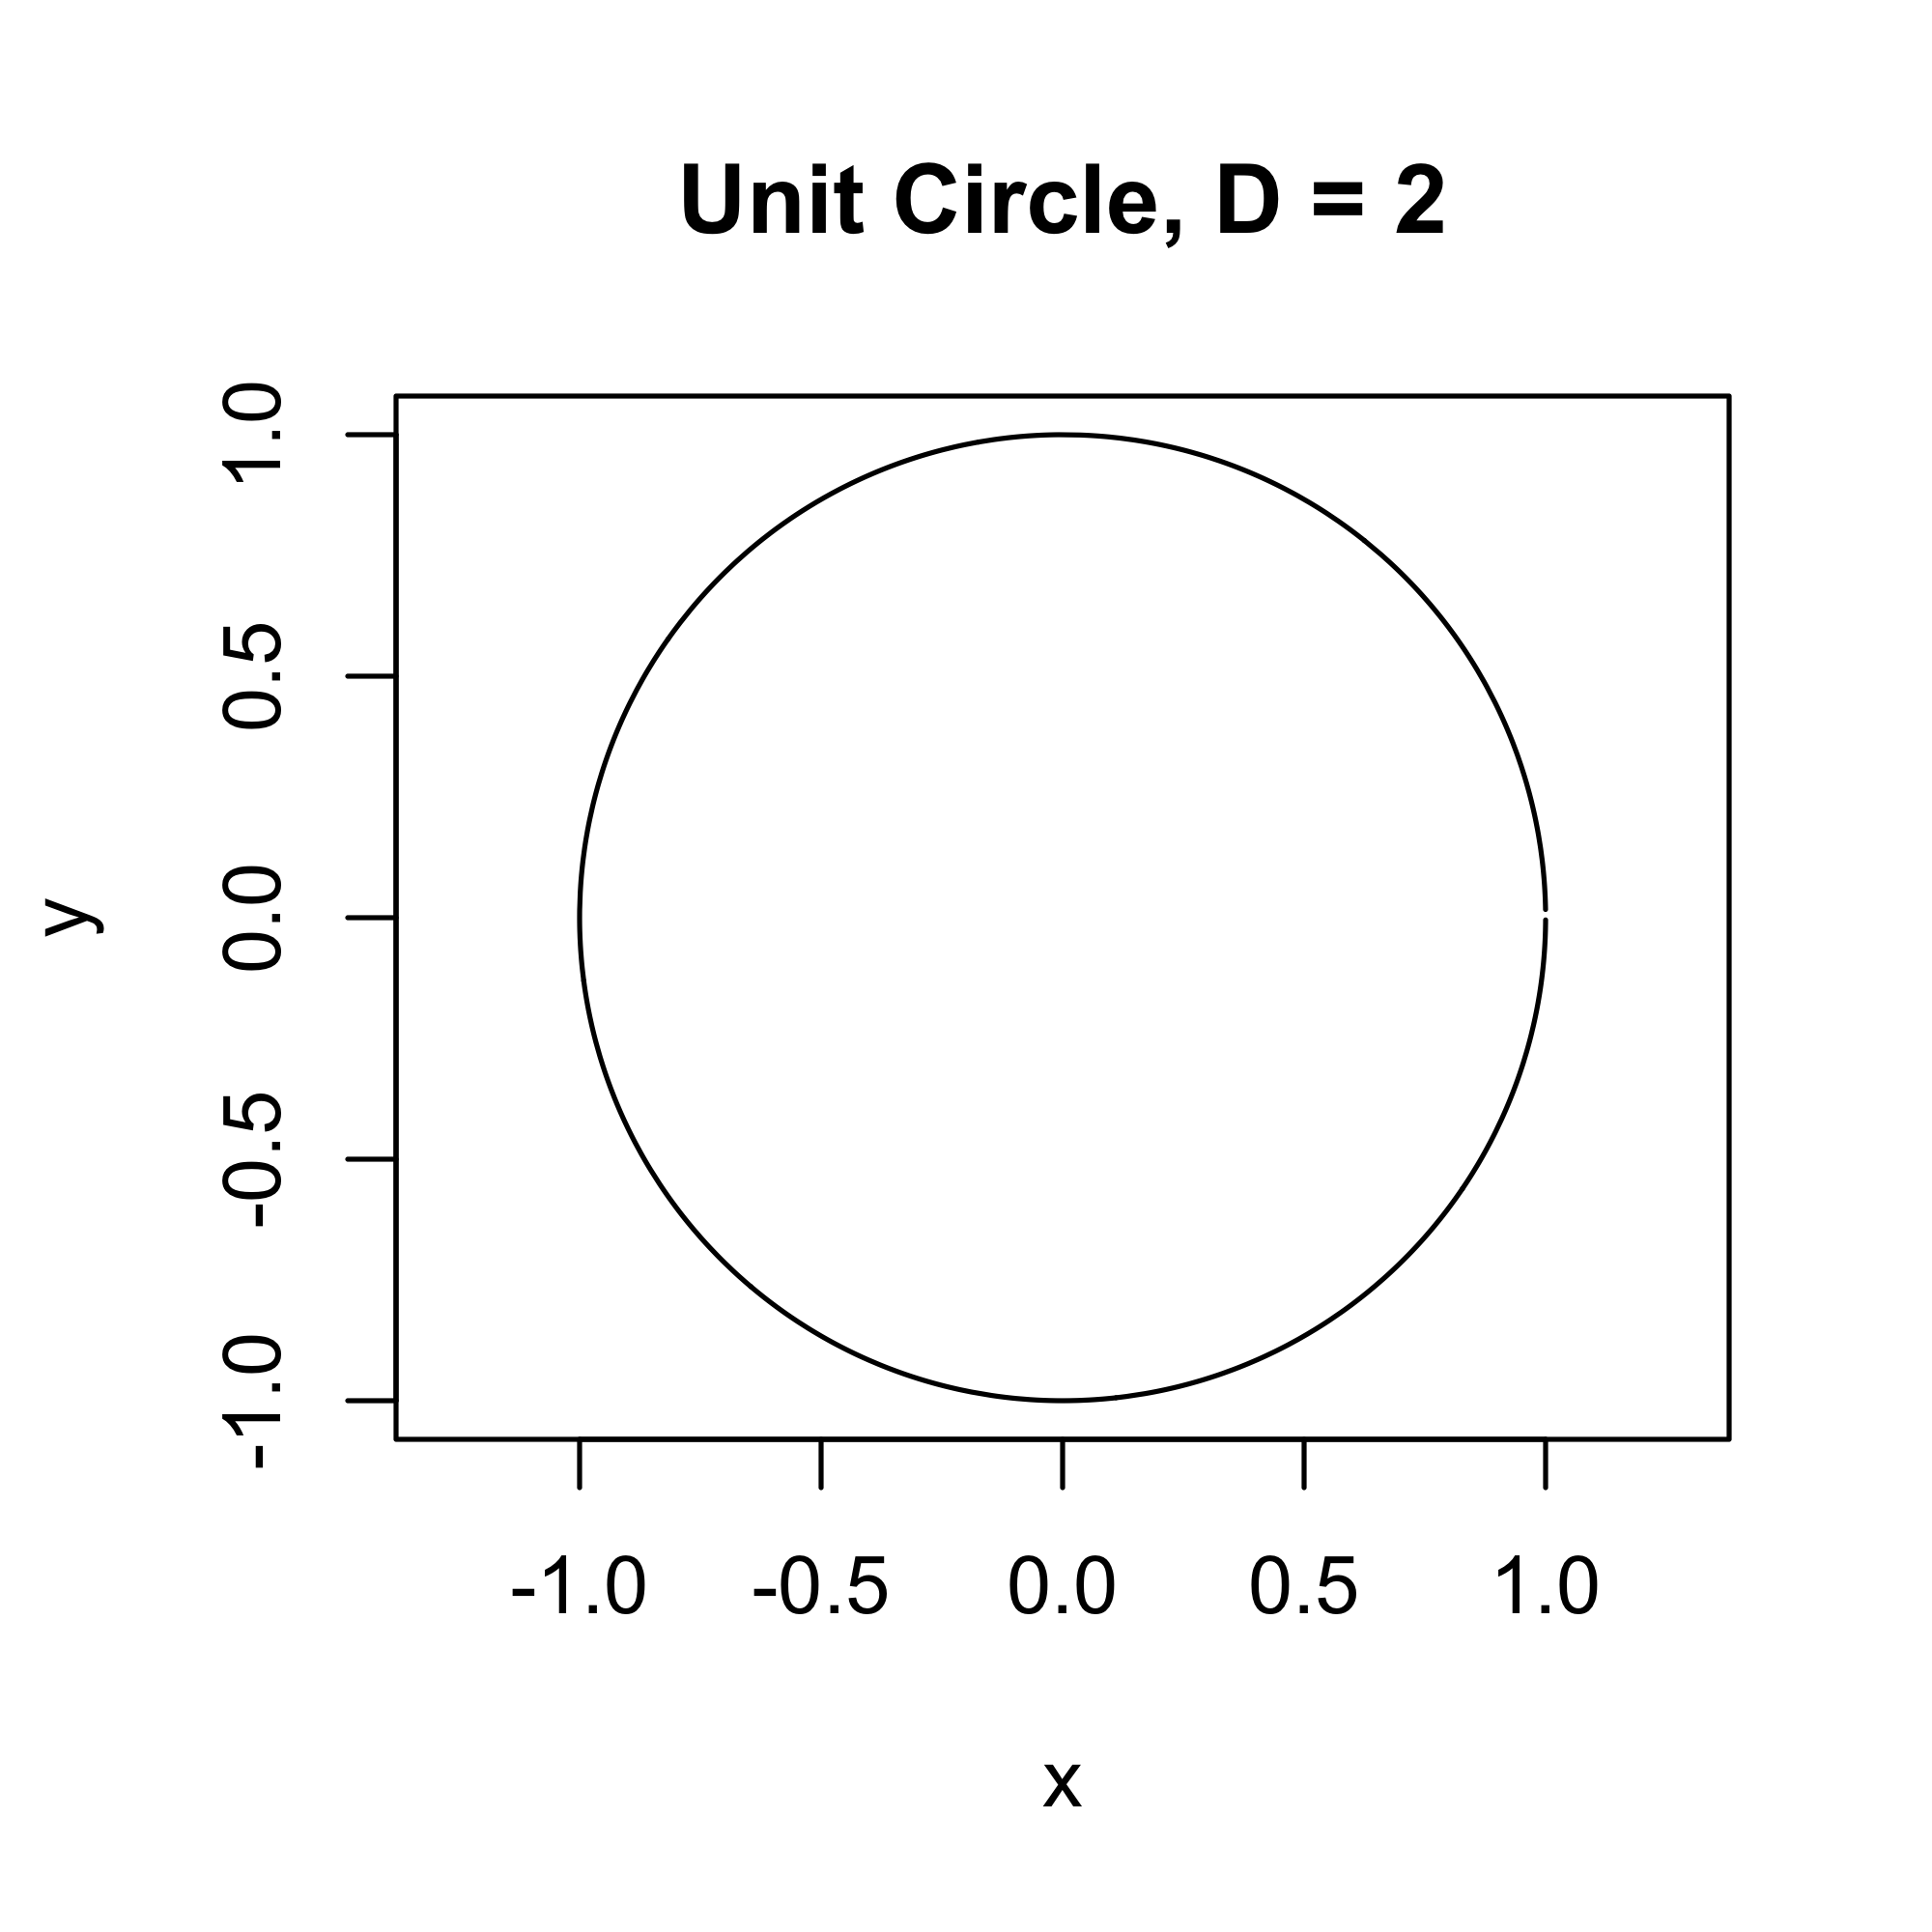
\includegraphics[width=9cm]{unit_circle_D2}}}%
  \hfill
  \subfloat[\centering $D = 3$]{{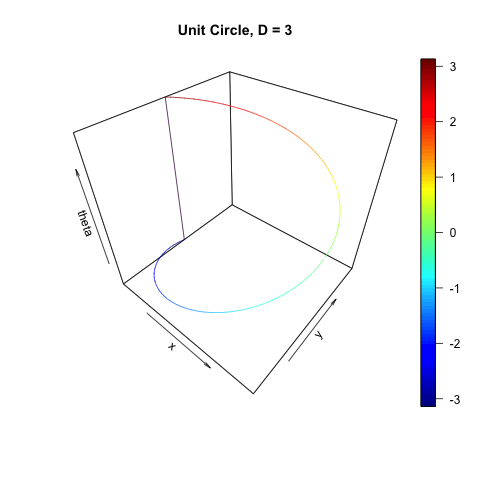
\includegraphics[width=9cm]{unit_circle_D3}}}
  \caption{Augmenting the Unit Circle}
  \label{fig:unit_circle_augmentation}
\end{figure}

\zielinski{The simulation results shown below use partial results run on my computer.}

A factorial design is used to run the simulation studies, with the factor levels set as follows:
\begin{itemize}
  \item $\alpha, \beta, \zeta \in \left\{0, 0.1, 0.25, 0.5, 1.0, 2.0\right\}$
  \item Study duration: $\left\{1, 2, 5, 10\right\}$
  \item Interval between images: $\left\{0.1, 0.25, 0.5, 1\right\}$
  \item Sample size: $\left\{1000, 10000\right\}$
  \item Longitudinal change model: Constant, Linear, Quadratic, Sinusoidal
\end{itemize}

Thus, each embedding map is simulated a total of 27,648 times. All code required to reproduce the simulation results and the associated figures is provided at \texttt{https://github.com/rjzielinski/lpme-project}.

Visualizations of the results from some of the simulation cases, truncated for concision to include only integer-valued time points, are shown in Figures \ref{fig:sim_case1}, \ref{fig:sim_case4} and \ref{fig:sim_case6}. Informally, the performance of each estimation method can be observed by considering the proximity of each method's estimated manifold to the true manifold (shown in red) over time. Thus, in Figure \ref{fig:sim_case1}, we see that the LPME-estimated manifold bears the closest resemblance to the true manifold underlying the data, while the manifolds estimated by PME and the principal curve method show greater responses to temporary random fluctuations in the data at each time point.

\zielinski{It may be necessary to put some of the simulation figures in an appendix. Additionally, the figures are still very much a work in progress and are serving more of a placeholder status at the moment. Any suggestions regarding how to improve the clarity and depth perception of the figures would be greatly appreciated!}

\begin{table}
  \centering
  \begin{tabular}{|c c c c c c c c c c|}
    \hline
    Method & Case 1 & Case 2 & Case 3 & Case 4 & Case 5 & Case 6 & Case 7 & Case 8 & Case 9 \\
    \hline
    Data & 0.240 (0.346) & 0.489 (0.399) & N/A & 19.2 (48.7) & 0.906 (0.735) & 1.20 (3.16) & N/A & N/A & N/A \\
    LPME & 0.166 (0.668) & 0.324 (0.327) & N/A & 11.8 (31.1) & 0.633 (0.692) & 1.11 (2.61) & N/A & N/A & N/A \\
    PME & 0.265 (0.430) & 0.615 (0.850) & N/A & 19.2 (48.7) & 0.918 (0.831) & 1.26 (3.17) & N/A & N/A & N/A \\
    PC/PS & 0.209 (0.342) & 0.557 (0.319) & N/A & 19.2 (48.7) & 0.863 (0.670) & 0.965 (1.17) & N/A & N/A & N/A \\
    \hline
  \end{tabular}
  \caption{MSD Comparison to True Values, Mean (SD).}
  \label{table:simulation_results_mean}
\end{table}

\begin{table}
  \centering
  \begin{tabular}{|c c c c c c c c c c|}
    \hline
    Method & Case 1 & Case 2 & Case 3 & Case 4 & Case 5 & Case 6 & Case 7 & Case 8 & Case 9 \\
    \hline
    Data & 0.134 (0.232) & 0.382 (0.649) & N/A & 3.37 (15.7) & 0.729 (1.29) & 0.328 (0.742) & N/A & N/A & N/A \\
    LPME & 0.0661 (0.119) & 0.236 (0.438) & N/A & 3.10 (9.54) & 0.370 (0.889) & 0.364 (0.671) & N/A & N/A & N/A \\
    PME & 0.117 (0.281) & 0.463 (0.668) & N/A & 3.34 (15.6) & 0.675 (1.31) & 0.369 (0.680) & N/A & N/A & N/A \\
    PC/PS & 0.110 (0.214) & 0.471 (0.467) & N/A & 3.33 (15.7) & 0.691 (1.18) & 0.607 (0.329) & N/A & N/A & N/A \\
    \hline
  \end{tabular}
  \caption{MSD Comparison to True Values, Median (IQR).}
  \label{table:simulation_results_median}
\end{table}

\begin{figure}%
  \centering
  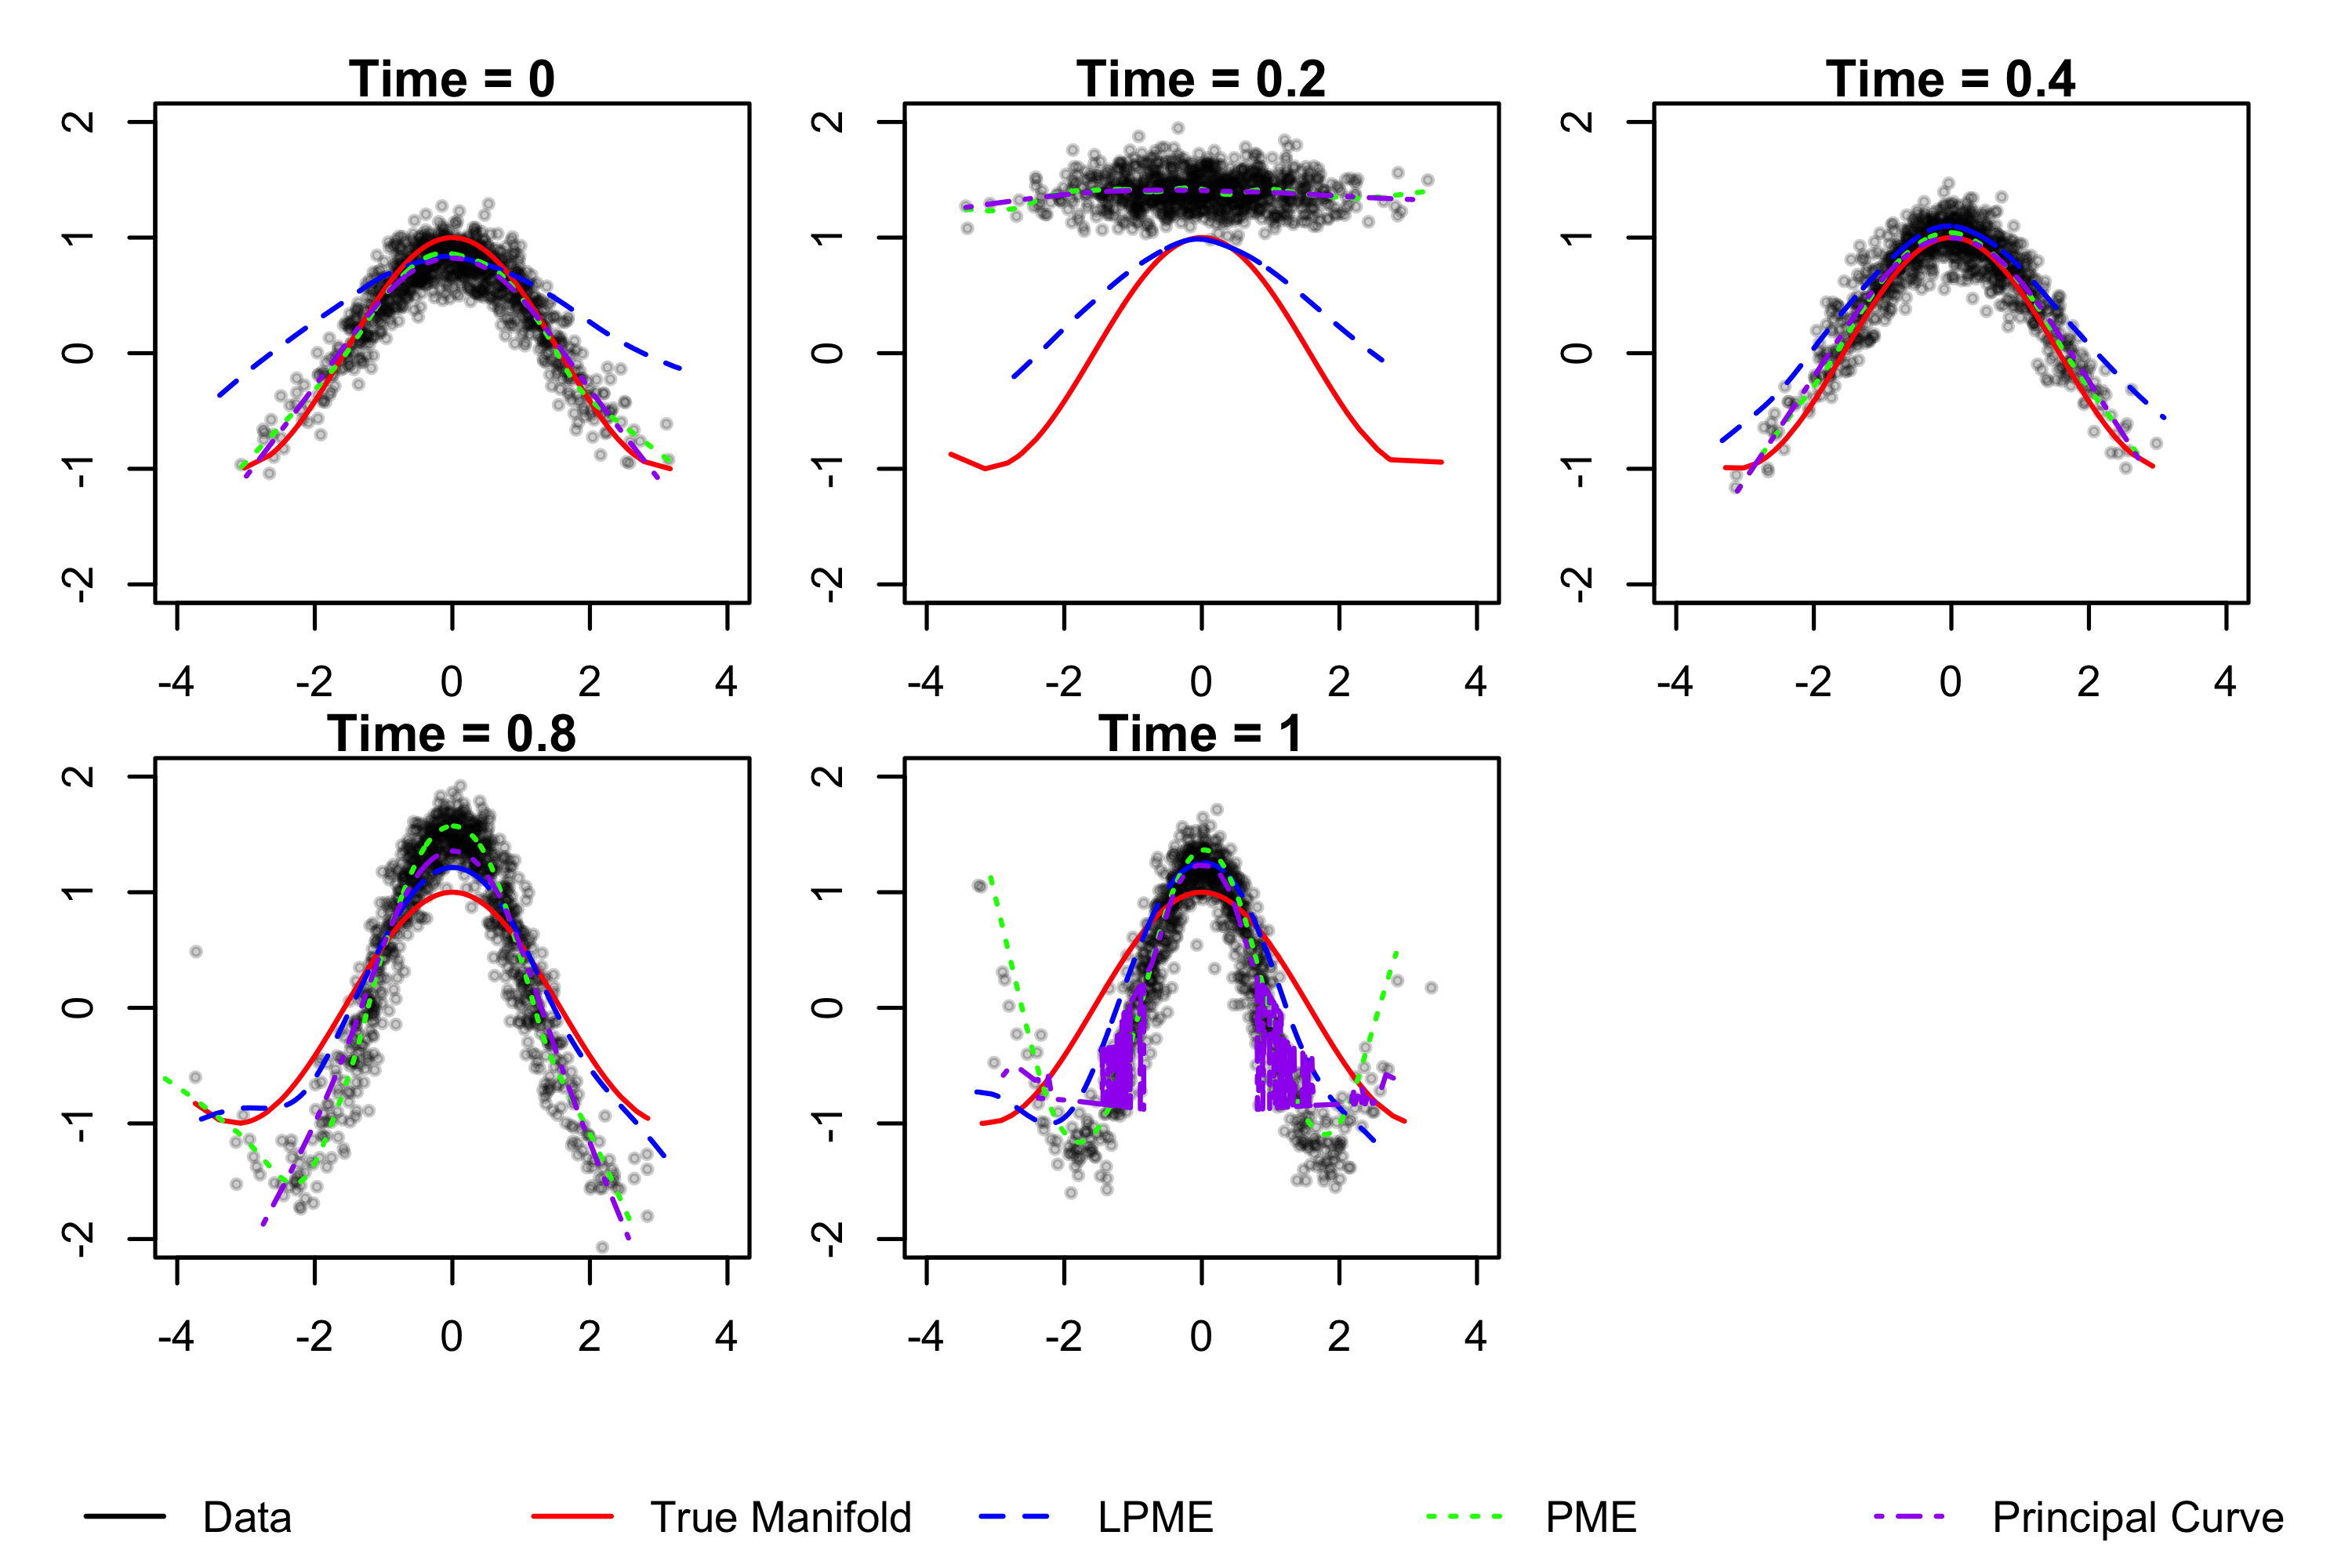
\includegraphics[width=\textwidth]{sim_case1}
  \caption{Simulation Case 1}
  \label{fig:sim_case1}
\end{figure}

\begin{figure}
  \centering
  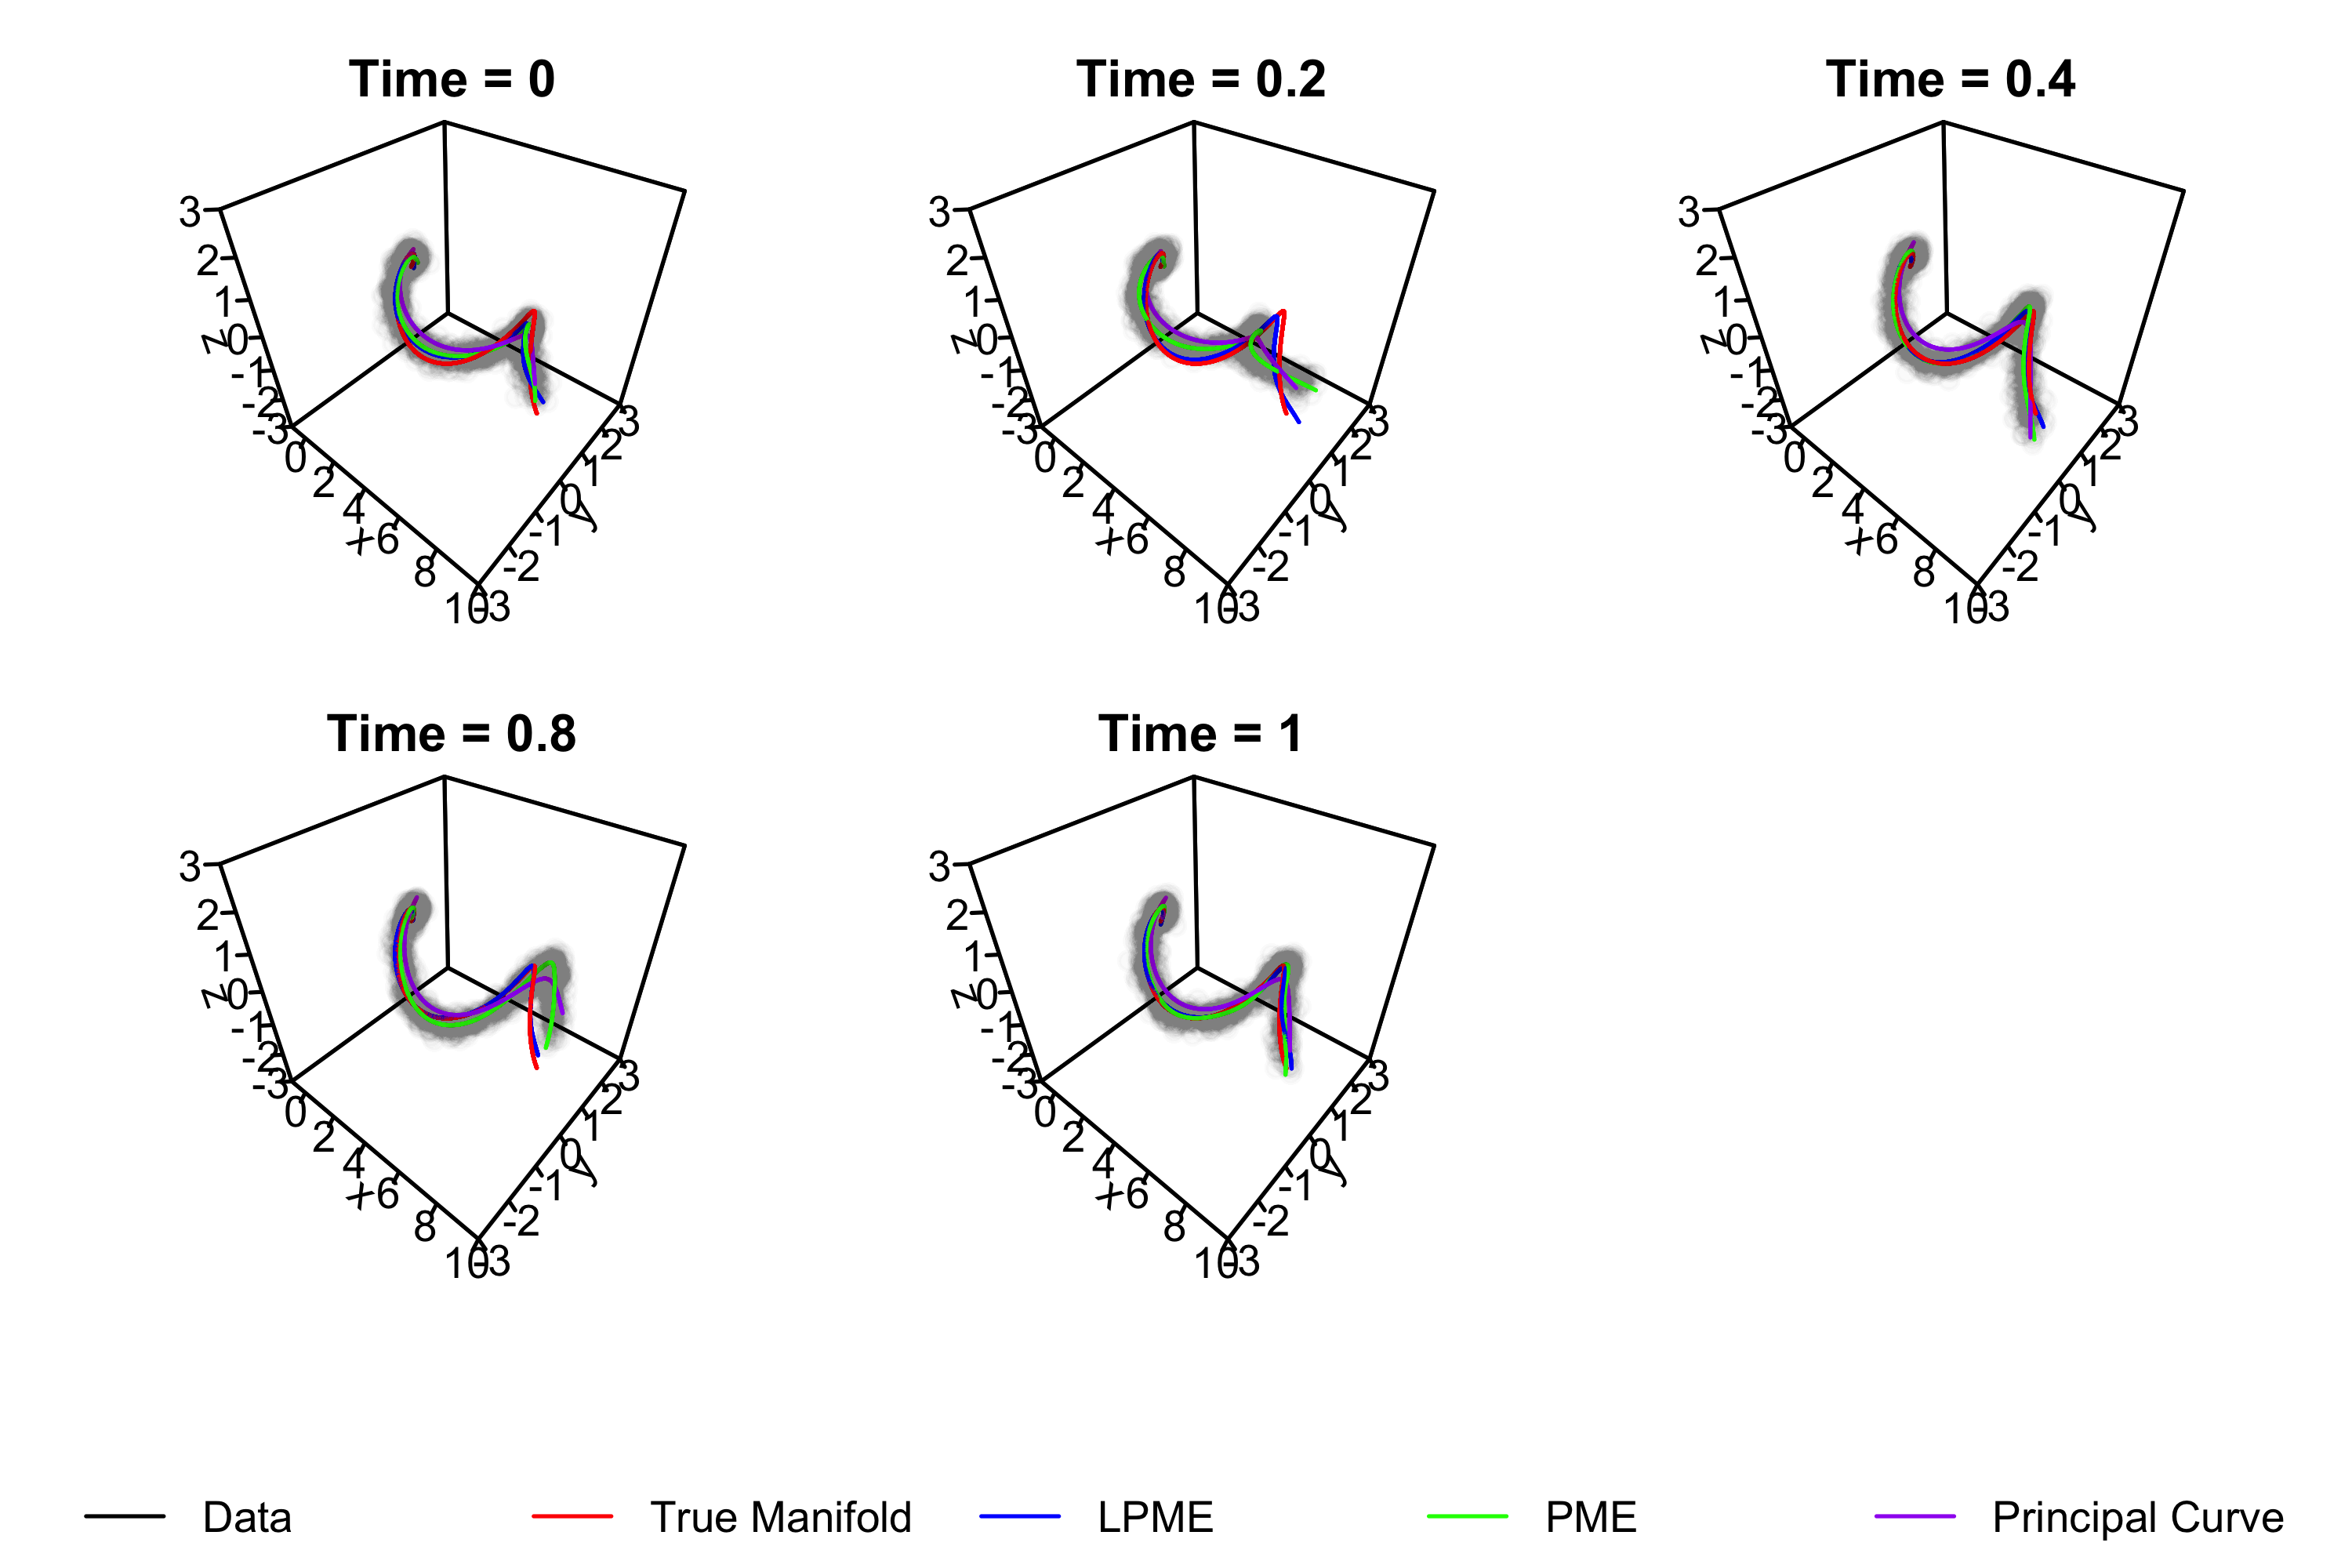
\includegraphics[width=\textwidth]{sim_case5}
  \caption{Simulation Case 4}
  \label{fig:sim_case4}
\end{figure}

\begin{figure}
  \centering
  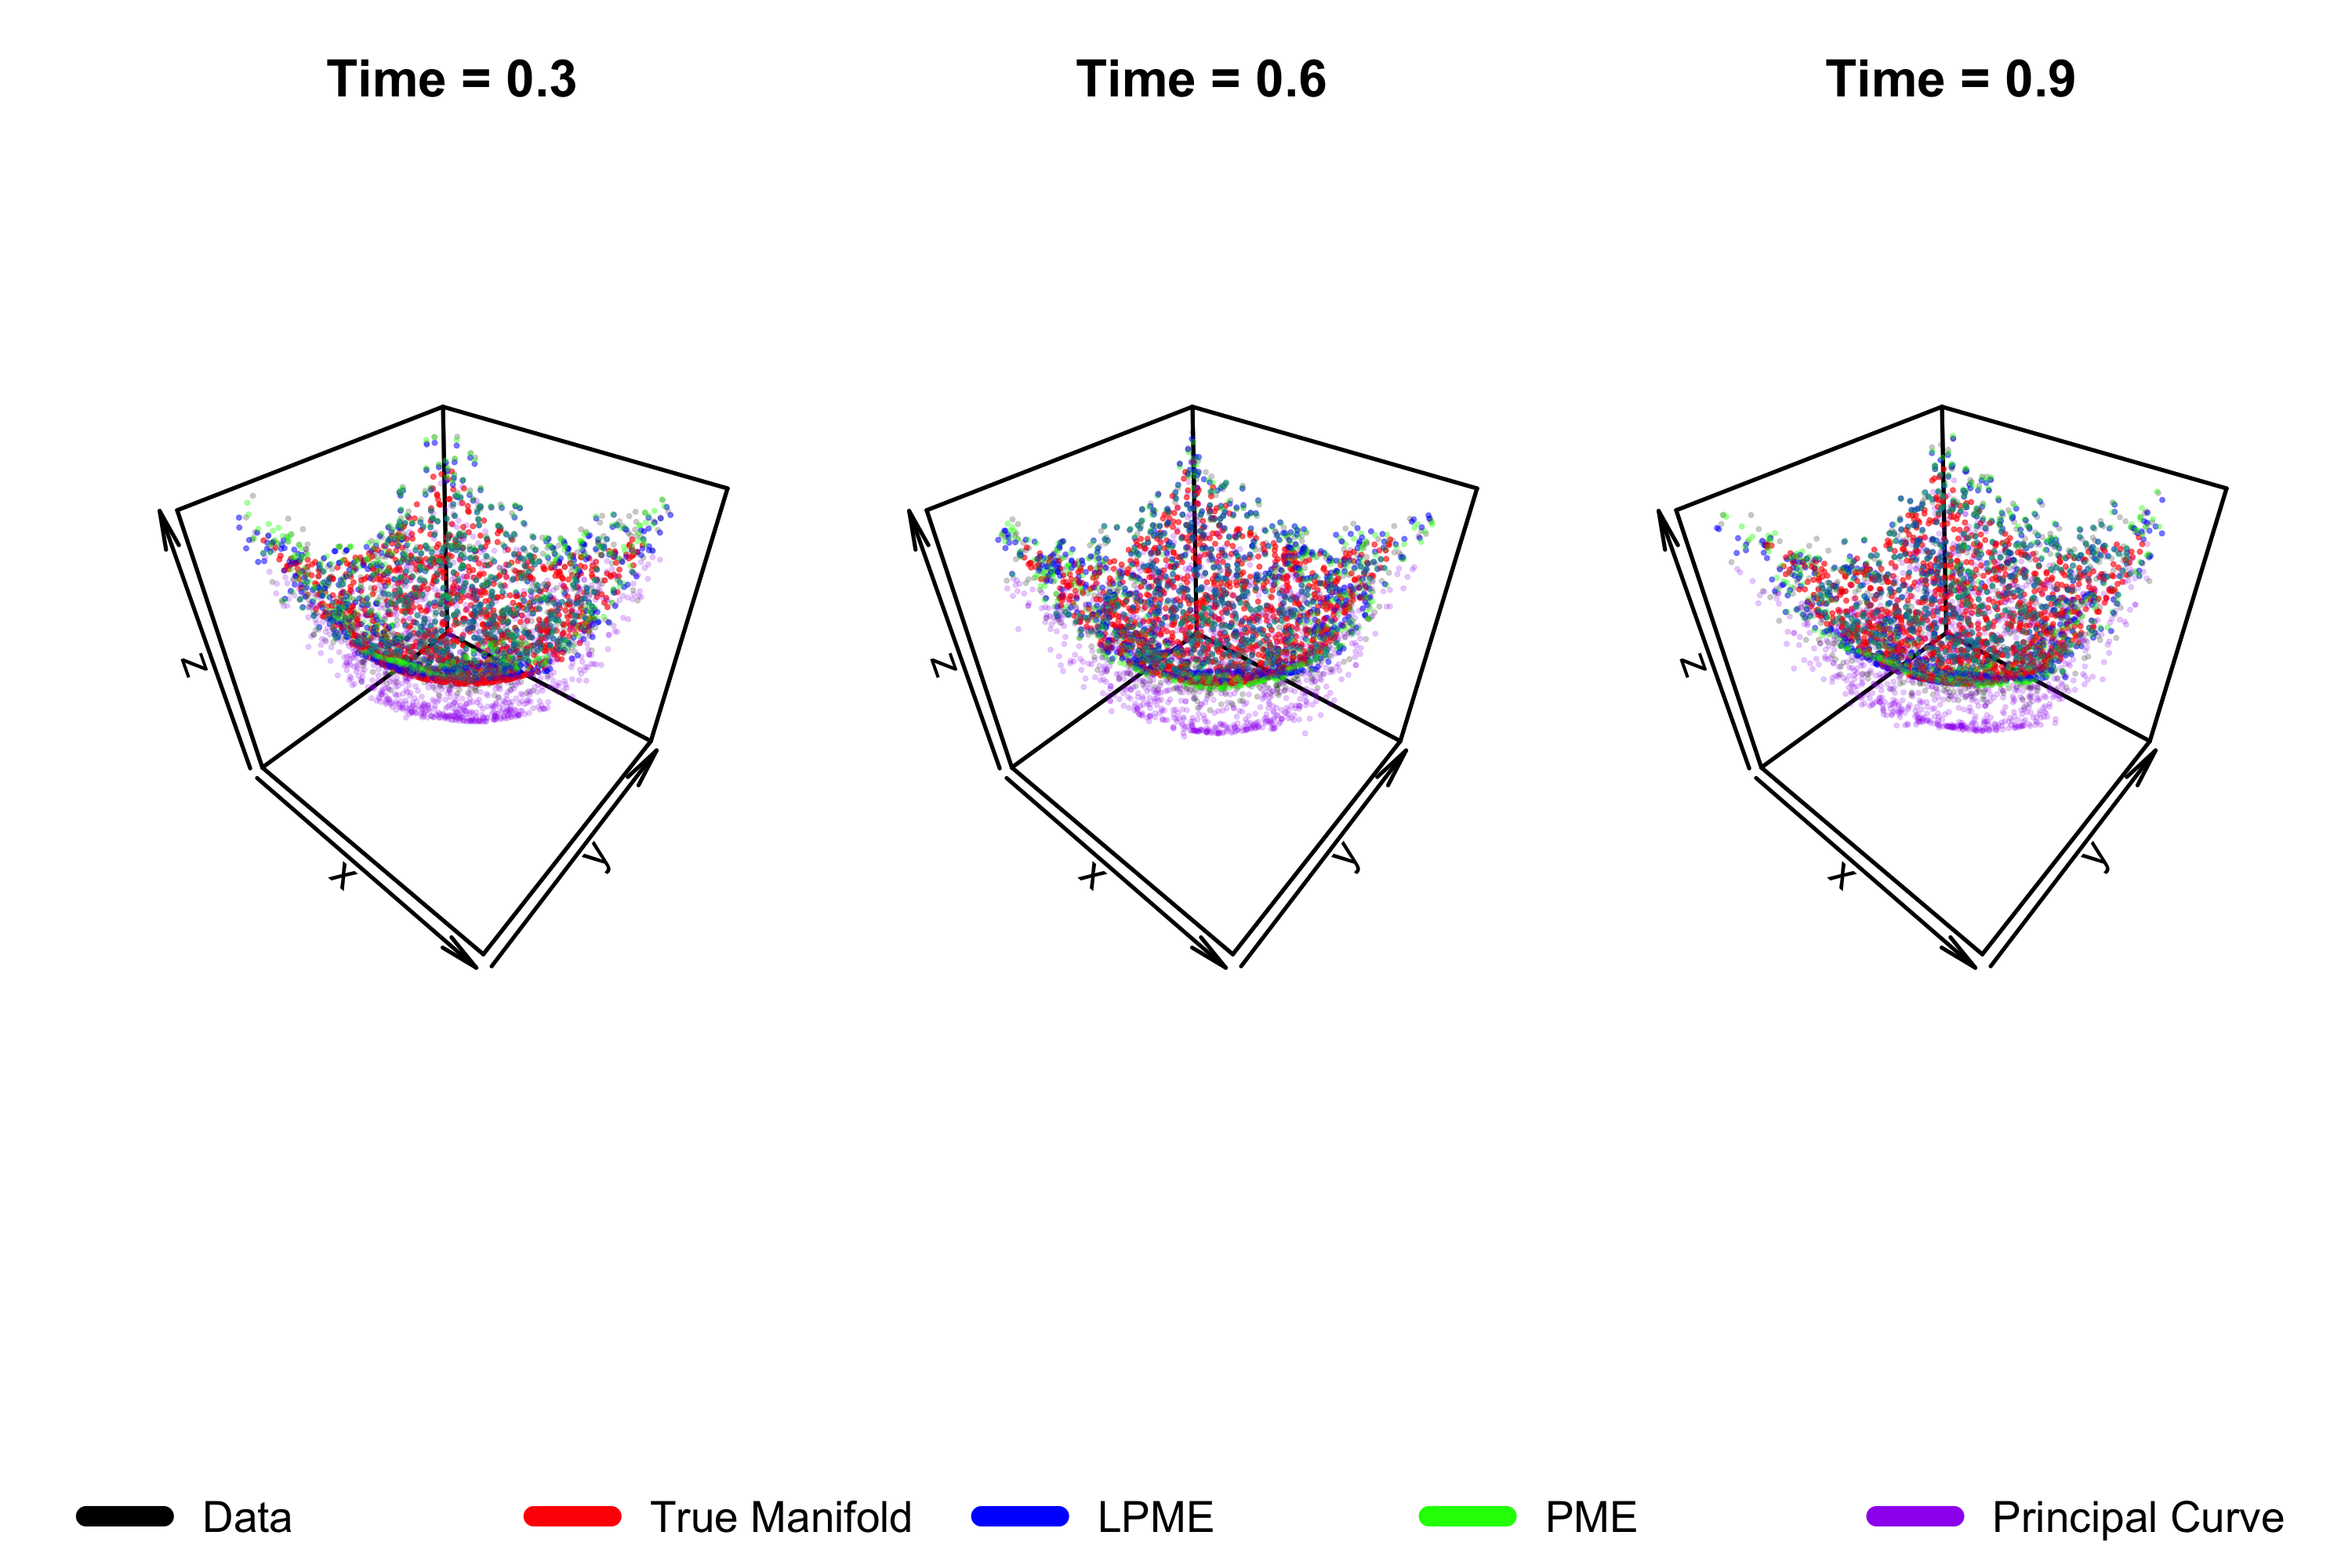
\includegraphics[width=\textwidth]{sim_case7}
  \caption{Simulation Case 6}
  \label{fig:sim_case6}
\end{figure}

The mean, median, and standard deviation of the mean squared distance from the true underlying manifold values for the estimates of each approach, as well as for the data itself, are shown in Tables \ref{table:simulation_results_mean} and \ref{table:simulation_results_median}. Because the PME, principal curve, and principal surface methods each attempt to estimate the manifold in question at each individual time point without allowing other time points to inform these estimates, they should result in similar deviations from the true underlying manifold, with differences in error resulting primarily from differing performances in fitting to the observed data. Meanwhile, because the LPME approach accounts for all time points simultaneously, this approach should result in lower mean squared distance values.

The result summaries indicate that in most cases, LPME provides a substantial improvement in performance over the PME and principal curve approaches when estimating the underlying manifold. As seen clearly in Figure \ref{fig:sim_case1}, while the structure of the simulated data changes noticeably between time points, the LPME estimates, shown in blue, remain relatively stable over time. This contrasts to the estimates found by the PME and principal curve approaches, which are highly sensitive to the data observed at each given time point, as expected. This ultimately results in the LPME estimates remaining closer to the true underlying manifold, shown in red. Similar results hold in most of the other simulation cases.

\zielinski{It is key to note here that the MSD values shown in these tables are comparing the various models' projections onto the estimated manifold to the true values underlying the data the models are fit on. This means that a model that performs well using this metric may not perform well when comparing the data to the model's projections onto the manifold. In fact, if there is a high level of inter-observation noise, then we should expect an estimated manifold that closely follows the true underlying manifold to show a relatively poor fit to the data at any given time point.

This largely explains why PME does not usually show better performance than the PC/PS methods using this metric - both approaches are trying to estimate a curve or surface using the data available at a given time point, which may have noise introduced that increases the distance to the true manifold. When comparing the fit of the PME and PC methods to the simulated data, PME tends to show improvement in the median MSD, with elevated mean MSD levels compared to principal curves.}

\section{Application}

As discussed previously, meaningful between-image error in estimates of subcortical structures is introduced during the process of segmenting MRI images. This section demonstrates how the LPME algorithm may be used to mitigate the effects of such noise on further analysis using these estimates. To achieve this, we used MRI data collected through the ADNI study, a longitudinal observational study with the goal of identifying imaging biomarkers to assess the progression of Alzheimer's disease (AD). 

While the original study included 200 cognitively healthy elderly individuals, 400 with mild cognitive impairment, and 200 with AD, for the purposes of demonstration we used $T_1$-weighted structural MRI images from eight study participants in the cognitively normal group (\cite{jack2008adni}). Follow-up duration for these participants ranged between approximately 16 months to 48 months, with imaging scheduled to be conducted at six month intervals. Individuals from the cognitively normal group were selected because drastic changes in the volume and shape of subcortical structures over the course of the study follow-up duration would be unexpected. Under this assumption, we attribute volumetric changes in a given structure to error introduced by the study procedure or the image segmentation process. Due to the changes experienced by those with Alzheimer's disease, we focused on the hippocampi of the selected individuals. 

Images were processed using FSL and ANTs via the \texttt{fslr} and \texttt{ANTsR} packages in \texttt{R}. Specifically, ANTs was used for bias correcting the images, and the FIRST method in FSL was used for image segmentation. Following image segmentation, the surfaces of each hippocampus were identified by finding the extreme voxels in each dimension with nonzero intensity readings. The estimated hippocampus surface positions were then standardized to a maximum distance of one from the origin in Euclidean space and centered around the origin.

Provide a brief summary of the results of the model fitting here, along with the related figures.

\section{Discussion}



\subsection*{Contributions}

\subsection*{Limitations}

\begin{enumerate}
  \item Algorithm assumes stability in shape over time.
  \item Algorithm initialization is sensitive to magnitude of change between time points.
  \item Computation time.
\end{enumerate}

Future Work:

\nocite{*}
%\bibliographystyle{plain}
%\bibliography{references}
\printbibliography

\end{document}
